\documentclass[]{article}
\usepackage{lmodern}
\usepackage{amssymb,amsmath}
\usepackage{ifxetex,ifluatex}
\usepackage{fixltx2e} % provides \textsubscript
\ifnum 0\ifxetex 1\fi\ifluatex 1\fi=0 % if pdftex
  \usepackage[T1]{fontenc}
  \usepackage[utf8]{inputenc}
\else % if luatex or xelatex
  \ifxetex
    \usepackage{mathspec}
  \else
    \usepackage{fontspec}
  \fi
  \defaultfontfeatures{Ligatures=TeX,Scale=MatchLowercase}
\fi
% use upquote if available, for straight quotes in verbatim environments
\IfFileExists{upquote.sty}{\usepackage{upquote}}{}
% use microtype if available
\IfFileExists{microtype.sty}{%
\usepackage[]{microtype}
\UseMicrotypeSet[protrusion]{basicmath} % disable protrusion for tt fonts
}{}
\PassOptionsToPackage{hyphens}{url} % url is loaded by hyperref
\usepackage[unicode=true]{hyperref}
\hypersetup{
            pdftitle={The specificity of statistical learning},
            pdfauthor={Ansgar Endress},
            pdfkeywords={Keywords},
            pdfborder={0 0 0},
            breaklinks=true}
\urlstyle{same}  % don't use monospace font for urls
\usepackage[margin=1in]{geometry}
\usepackage{natbib}
\bibliographystyle{plainnat}
\usepackage{color}
\usepackage{fancyvrb}
\newcommand{\VerbBar}{|}
\newcommand{\VERB}{\Verb[commandchars=\\\{\}]}
\DefineVerbatimEnvironment{Highlighting}{Verbatim}{commandchars=\\\{\}}
% Add ',fontsize=\small' for more characters per line
\usepackage{framed}
\definecolor{shadecolor}{RGB}{248,248,248}
\newenvironment{Shaded}{\begin{snugshade}}{\end{snugshade}}
\newcommand{\KeywordTok}[1]{\textcolor[rgb]{0.13,0.29,0.53}{\textbf{#1}}}
\newcommand{\DataTypeTok}[1]{\textcolor[rgb]{0.13,0.29,0.53}{#1}}
\newcommand{\DecValTok}[1]{\textcolor[rgb]{0.00,0.00,0.81}{#1}}
\newcommand{\BaseNTok}[1]{\textcolor[rgb]{0.00,0.00,0.81}{#1}}
\newcommand{\FloatTok}[1]{\textcolor[rgb]{0.00,0.00,0.81}{#1}}
\newcommand{\ConstantTok}[1]{\textcolor[rgb]{0.00,0.00,0.00}{#1}}
\newcommand{\CharTok}[1]{\textcolor[rgb]{0.31,0.60,0.02}{#1}}
\newcommand{\SpecialCharTok}[1]{\textcolor[rgb]{0.00,0.00,0.00}{#1}}
\newcommand{\StringTok}[1]{\textcolor[rgb]{0.31,0.60,0.02}{#1}}
\newcommand{\VerbatimStringTok}[1]{\textcolor[rgb]{0.31,0.60,0.02}{#1}}
\newcommand{\SpecialStringTok}[1]{\textcolor[rgb]{0.31,0.60,0.02}{#1}}
\newcommand{\ImportTok}[1]{#1}
\newcommand{\CommentTok}[1]{\textcolor[rgb]{0.56,0.35,0.01}{\textit{#1}}}
\newcommand{\DocumentationTok}[1]{\textcolor[rgb]{0.56,0.35,0.01}{\textbf{\textit{#1}}}}
\newcommand{\AnnotationTok}[1]{\textcolor[rgb]{0.56,0.35,0.01}{\textbf{\textit{#1}}}}
\newcommand{\CommentVarTok}[1]{\textcolor[rgb]{0.56,0.35,0.01}{\textbf{\textit{#1}}}}
\newcommand{\OtherTok}[1]{\textcolor[rgb]{0.56,0.35,0.01}{#1}}
\newcommand{\FunctionTok}[1]{\textcolor[rgb]{0.00,0.00,0.00}{#1}}
\newcommand{\VariableTok}[1]{\textcolor[rgb]{0.00,0.00,0.00}{#1}}
\newcommand{\ControlFlowTok}[1]{\textcolor[rgb]{0.13,0.29,0.53}{\textbf{#1}}}
\newcommand{\OperatorTok}[1]{\textcolor[rgb]{0.81,0.36,0.00}{\textbf{#1}}}
\newcommand{\BuiltInTok}[1]{#1}
\newcommand{\ExtensionTok}[1]{#1}
\newcommand{\PreprocessorTok}[1]{\textcolor[rgb]{0.56,0.35,0.01}{\textit{#1}}}
\newcommand{\AttributeTok}[1]{\textcolor[rgb]{0.77,0.63,0.00}{#1}}
\newcommand{\RegionMarkerTok}[1]{#1}
\newcommand{\InformationTok}[1]{\textcolor[rgb]{0.56,0.35,0.01}{\textbf{\textit{#1}}}}
\newcommand{\WarningTok}[1]{\textcolor[rgb]{0.56,0.35,0.01}{\textbf{\textit{#1}}}}
\newcommand{\AlertTok}[1]{\textcolor[rgb]{0.94,0.16,0.16}{#1}}
\newcommand{\ErrorTok}[1]{\textcolor[rgb]{0.64,0.00,0.00}{\textbf{#1}}}
\newcommand{\NormalTok}[1]{#1}
\usepackage{longtable,booktabs}
% Fix footnotes in tables (requires footnote package)
\IfFileExists{footnote.sty}{\usepackage{footnote}\makesavenoteenv{long table}}{}
\usepackage{graphicx,grffile}
\makeatletter
\def\maxwidth{\ifdim\Gin@nat@width>\linewidth\linewidth\else\Gin@nat@width\fi}
\def\maxheight{\ifdim\Gin@nat@height>\textheight\textheight\else\Gin@nat@height\fi}
\makeatother
% Scale images if necessary, so that they will not overflow the page
% margins by default, and it is still possible to overwrite the defaults
% using explicit options in \includegraphics[width, height, ...]{}
\setkeys{Gin}{width=\maxwidth,height=\maxheight,keepaspectratio}
\IfFileExists{parskip.sty}{%
\usepackage{parskip}
}{% else
\setlength{\parindent}{0pt}
\setlength{\parskip}{6pt plus 2pt minus 1pt}
}
\setlength{\emergencystretch}{3em}  % prevent overfull lines
\providecommand{\tightlist}{%
  \setlength{\itemsep}{0pt}\setlength{\parskip}{0pt}}
\setcounter{secnumdepth}{5}
% Redefines (sub)paragraphs to behave more like sections
\ifx\paragraph\undefined\else
\let\oldparagraph\paragraph
\renewcommand{\paragraph}[1]{\oldparagraph{#1}\mbox{}}
\fi
\ifx\subparagraph\undefined\else
\let\oldsubparagraph\subparagraph
\renewcommand{\subparagraph}[1]{\oldsubparagraph{#1}\mbox{}}
\fi

% set default figure placement to htbp
\makeatletter
\def\fps@figure{htbp}
\makeatother

\newcommand{\citeeg}[1]{\cite<e.g.,>[]{#1}}
\newcommand{\cites}[1]{\citeauthor{#1}'s \citeyear{#1}}
\newcommand{\T}{{\em t\/}}
\newcommand{\F}{{\em F\/}}
\newcommand{\Z}{{\em Z\/}}
\newcommand{\p}{{\em p\/}}
\newcommand{\M}{{\em M\/}}
\newcommand{\SD}{{\em SD\/}}
\newcommand{\SE}{{\em SE\/}}
\newcommand{\D}{Cohen's {\em d\/}}
\newcommand{\CI}{$CI_{.95}$}
\newcommand{\et}{$\eta^2$}
\newcommand{\etp}{$\eta_p^2$}
\renewcommand{\U}{{\em U\/}}
\newcommand{\W}{{\em W\/}}
\newcommand{\I}{\mathcal{I}}
\newcommand{\decay}{\mathcal{D}}

\newcommand{\N}{{\mathbf N}}                   %Non-negative integers
\newcommand{\R}{{\mathbf R}}                   %Reals


\newcommand{\colorize}[1]{{\color{red}{#1}}}

% Insert sub-figures without sub-captions but labeling the sub-figures
\newcommand{\includesubgraphics}[2]{
  \begin{subfigure}[a][][t]{.9\textwidth}
    
    {\Large \bf #1 \vspace{-\baselineskip}} 
    
    \hspace{1em}\includegraphics[width=0.9\linewidth]{#2} 
  \end{subfigure}   
}
\usepackage{booktabs}
\usepackage{longtable}
\usepackage{array}
\usepackage{multirow}
\usepackage{wrapfig}
\usepackage{float}
\usepackage{colortbl}
\usepackage{pdflscape}
\usepackage{tabu}
\usepackage{threeparttable}
\usepackage{threeparttablex}
\usepackage[normalem]{ulem}
\usepackage{makecell}
\usepackage{xcolor}

\title{The specificity of statistical learning}
\author{Ansgar Endress}
\date{}

\begin{document}
\maketitle
\begin{abstract}
Statistical Learning exists in many domains and species. It might be
particularly crucial for the earliest stages of word learning, for
example for recovering word-like chunks from fluent speech. However,
other forms of associative learning are remarkably tuned to the
ecological constraints of the learning situation. Here, we show that
Statistical Learning is similarly constrained. It predominantly operates
in continuous speech sequences similar to those used in prior
experiments, but not in discrete chunk sequences similar to those likely
encountered during language acquisition (due to the prosodic
organization of language). Conversely, when exposed to continuous
sequence in a memory recall experiment, participants tend to produce
low-probability sequences because, to the extent that they remember any
items at all, they initiate their productions at random positions in the
sequence rather than at the onsets of statistically defined chunks. In
contrast, familiarization with discrete sequences produces reliable
memories of actual, high-probability forms. This dissociation between
Statistical Learning and memory suggests that Statistical Learning might
have a specialized role when distributional information can be
accumulated (e.g., for predictive processing), and that it is separable
from the (declarative) memory mechanisms needed to acquire words.
\end{abstract}

{
\setcounter{tocdepth}{5}
\tableofcontents
}
\begin{Shaded}
\begin{Highlighting}[]
\CommentTok{# Extract R file to accelarate segmentation}

\NormalTok{knitr}\OperatorTok{::}\KeywordTok{purl}\NormalTok{ (}\StringTok{'segmentation_recall_combined.Rmd'}\NormalTok{, }
      \StringTok{'segmentation_recall_combined.R'}\NormalTok{)}
\end{Highlighting}
\end{Shaded}

\section{House keeping}\label{house-keeping}

In the analyses below, we use the following parameters:

\begin{longtable}[]{@{}ll@{}}
\toprule
\begin{minipage}[b]{0.03\columnwidth}\raggedright\strut
Name\strut
\end{minipage} & \begin{minipage}[b]{0.92\columnwidth}\raggedright\strut
Value\strut
\end{minipage}\tabularnewline
\midrule
\endhead
\begin{minipage}[t]{0.03\columnwidth}\raggedright\strut
ANALYZED.DATA.SETS\strut
\end{minipage} & \begin{minipage}[t]{0.92\columnwidth}\raggedright\strut
TRUE\strut
\end{minipage}\tabularnewline
\begin{minipage}[t]{0.03\columnwidth}\raggedright\strut
ANALYZED.DATA.SETS\strut
\end{minipage} & \begin{minipage}[t]{0.92\columnwidth}\raggedright\strut
TRUE\strut
\end{minipage}\tabularnewline
\begin{minipage}[t]{0.03\columnwidth}\raggedright\strut
FILTER.SINGLE.SYLLABLES\strut
\end{minipage} & \begin{minipage}[t]{0.92\columnwidth}\raggedright\strut
FALSE\strut
\end{minipage}\tabularnewline
\begin{minipage}[t]{0.03\columnwidth}\raggedright\strut
FILTER.UNATTESTED.ITEMS\strut
\end{minipage} & \begin{minipage}[t]{0.92\columnwidth}\raggedright\strut
FALSE\strut
\end{minipage}\tabularnewline
\begin{minipage}[t]{0.03\columnwidth}\raggedright\strut
IGNORE.COL.PREFIXES\strut
\end{minipage} & \begin{minipage}[t]{0.92\columnwidth}\raggedright\strut
ITI\_\strut
\end{minipage}\tabularnewline
\begin{minipage}[t]{0.03\columnwidth}\raggedright\strut
IGNORE.COL.PREFIXES\strut
\end{minipage} & \begin{minipage}[t]{0.92\columnwidth}\raggedright\strut
presTime\_\strut
\end{minipage}\tabularnewline
\begin{minipage}[t]{0.03\columnwidth}\raggedright\strut
IGNORE.COL.PREFIXES\strut
\end{minipage} & \begin{minipage}[t]{0.92\columnwidth}\raggedright\strut
ISI\_\strut
\end{minipage}\tabularnewline
\begin{minipage}[t]{0.03\columnwidth}\raggedright\strut
L.BAD.SUBJ.CPUTIME\strut
\end{minipage} & \begin{minipage}[t]{0.92\columnwidth}\raggedright\strut
list(c(subj = ``399612\_200413\_124119\_M056106.csv'', response =
``dalonigtbdophophi dalobdakabdarobigopachu''), c(subj =
``399612\_210517\_101428\_M070415.csv'', response = ``be cu di tu dara
pe gala du dopa,be cu di pe gala,be cu di pe gala bu dopa ,be cu di bu
dopa''), c(subj = ``399612\_210517\_100654\_M038010.csv'', response =
``takahsakakakaratatataikokokokotatakatakatakatakatakatakataka''),
c(subj = " 399612\_210517\_101201\_M048600.csv``, response
=''dabroobitalooki,bkuti2,golab``), c(subj
=''399612\_210524\_062929\_M059506.csv``,\strut
\end{minipage}\tabularnewline
\begin{minipage}[t]{0.03\columnwidth}\raggedright\strut
response = ``matikulatatitulapapitularimatitulaatitula''), c(subj =
``399612\_210524\_115845\_M067482.csv'', response = ``tu kalla ti palla
tuti kulla papi pu tu kalla ti palla tuti kulla papi pu''), c(subj =
``399612\_210524\_120014\_M099076.csv'', response =
``tutopitulakatutopitoolaka''), c(subj =
``399612\_210524\_120523\_M003515.csv'', response =
``papikuchi,butalapapikuchi,kukala,pikala,budharapikuchi,chupapikachubudarapi''))\strut
\end{minipage} & \begin{minipage}[t]{0.92\columnwidth}\raggedright\strut
\strut
\end{minipage}\tabularnewline
\begin{minipage}[t]{0.03\columnwidth}\raggedright\strut
PRINT.INDIVIDUAL.FIGURES\strut
\end{minipage} & \begin{minipage}[t]{0.92\columnwidth}\raggedright\strut
FALSE\strut
\end{minipage}\tabularnewline
\begin{minipage}[t]{0.03\columnwidth}\raggedright\strut
PRINT.INDIVIDUAL.PDFS\strut
\end{minipage} & \begin{minipage}[t]{0.92\columnwidth}\raggedright\strut
TRUE\strut
\end{minipage}\tabularnewline
\begin{minipage}[t]{0.03\columnwidth}\raggedright\strut
PRINT.INDIVIDUAL.TABLES\strut
\end{minipage} & \begin{minipage}[t]{0.92\columnwidth}\raggedright\strut
FALSE\strut
\end{minipage}\tabularnewline
\begin{minipage}[t]{0.03\columnwidth}\raggedright\strut
REMOVE.BAD.SUBJ\strut
\end{minipage} & \begin{minipage}[t]{0.92\columnwidth}\raggedright\strut
TRUE\strut
\end{minipage}\tabularnewline
\begin{minipage}[t]{0.03\columnwidth}\raggedright\strut
REMOVE.INCOMPLETE.SUBJ\strut
\end{minipage} & \begin{minipage}[t]{0.92\columnwidth}\raggedright\strut
FALSE\strut
\end{minipage}\tabularnewline
\begin{minipage}[t]{0.03\columnwidth}\raggedright\strut
RESEGMENT.RESPONSES\strut
\end{minipage} & \begin{minipage}[t]{0.92\columnwidth}\raggedright\strut
FALSE\strut
\end{minipage}\tabularnewline
\begin{minipage}[t]{0.03\columnwidth}\raggedright\strut
start.time\strut
\end{minipage} & \begin{minipage}[t]{0.92\columnwidth}\raggedright\strut
2021-06-01 19:18:06\strut
\end{minipage}\tabularnewline
\bottomrule
\end{longtable}

\clearpage

\section{Introduction}\label{introduction}

Associative learning is widespread and exists in many species and
domains
\citetext{\citealp{Aslin1998}; \citealp{Chen2015}; \citealp[Conway2005a;][]{Fiser2002}; \citealp{Hauser2001}; \citealp{Saffran-Science}; \citealp{Toro2005-backward}; \citealp{Turk-Browne2005}; \citealp{Turk-Browne-reversal}}.
This led to the conclusion that the computations for which it is
critical might be similarly widespread, a view that has been
particularly prominent in language acquisition
\citep{Aslin2012, Seidenberg2002, Thiessen2017}.

However, associative learning is also remarkably modular
\citep{Endress-duplications}. For example, humans have independent
associative learning abilities in superficially similar domains,
including the learning of associations of objects with landmarks
vs.~boundaries \citep{Doeller2008, Doeller2008a}, associations among
social vs.~non-social objects \citep{Tompson2019} and associations among
consonants vs.~vowels \citep{Bonatti2005}. Further, associative learning
abilities are generally not correlated across domains
\citep{Siegelman2015}.

Preferential associations between specific classes of stimuli abound
\citep{Seligman1970}, and can evolve in just 40 generations in fruit
flies \citep{Dunlap2014}. For example, rats readily associate tastes
with sickness and external events such as sounds or light flashes with
pain, but cannot (or only with great difficulty) associate taste with
pain or external events with sickness \citep{Garcia1974, Garcia1976}.
This pattern of associations reflects the likely ecological sources of
sickness vs.~pain (i.e., food vs.~external events). Critically, the
formation of taste-sickness associations (but not of other forms of
associations) is blocked in a suckling context for rats who have not
been exposed to solid food \citep{Martin1979, Alberts1984}, presumably
because avoidance of the only food source would be detrimental; in
contrast, minimal exposure to solid food re-establish taste-sickness
associations \citep{Gubernick1984}.

While such results suggest that, over evolutionary times, the
adaptiveness of associative learning is regulated by increasing or
decreasing its availability for specific classes of stimuli, it is less
clear if associative learning is specialized for specific computational
functions, or whether it is essentially a side effect of local neural
processing \citep[a ``spandrel'' in biological terms;][]{Gould1979},
that is sometimes adaptive, somtimes neutral and sometimes detrimentl.
Here, we address this issue in a domain where the importance of
associative learning has long been recognized: word learning. We suggest
that associative learning is critical for predicting speech material
under conditions where it can be predicted, but that it does not lead to
memory.

One of the most prominent cases for associative learning in language
acquisition is word segmentation. Speech is thought to be a continuous
signal, and before learners can commit any words to memory, they need to
learn where words start and where they end, respectively. One strategy
to find word boundaries relies on Transitional Probabilities (TPs) among
items, that is, the conditional probability of a syllable
\(\sigma_{i+1}\) given a preceeding syllable \(\sigma_{i+1}\),
\(P(\sigma_{i}\sigma_{i+1})/P(\sigma_{i})\). Early on, Shannon
\citep{Shannon1951} showed that human adults are sensitive to such
distributional information. Subsequent work conclusively demonstrated
that infants and non-human animals share this ability {[}XXX{]}, and
suggested that TPs can be extract using simple associative mechanisms
such as Hebbian learning \citep{Endress-TP-Model}.

However, a sensitivity to distributional information does not imply that
learners extract chunks that can be stored in memory. In fact, such as
sensitive is typically tested by comparing participants' preference for
high-TP items over low-TP items. It turns out that participants
sometimes prefer high-TP items thet have never seen or heard (and thus
could not have memorize) over low-TP items they have heard
\citep{Endress-Phantoms-Vision}, suggesting that associative learning
and memory for specific chunks may be dissociable. In fact, the types of
representations created by associative learning might well be different
from those used for linguistic stimuli
\citep{Endress-Phantoms-Vision, Fischer-Baum2011}, while associative
knowledge might be critical for predictive processing that is critical
for both language \citep{Levy2008, Trueswell1999} and other cognitive
processes (XXX).

Here, we test this idea, focusing on the conditions under which
associative learning operates and on the function it might have. To
elucidate the conditions under which associative learning operates, we
note that speech does not come as an continuous signal but rather as a
sequence of smaller units due to its prosodic organization
\citep{Beckman1986, Cutler1997, Nespor1986, Selkirk1986, Shattuck-Hufnagel1996}.
This prosodic organization is perceived in unfamiliar languages
\citep{Brentari2011, Endress-cross-seg, Fenlon2008, Pilon1981}, by
infants
\citetext{\citealp{Hirsh-Pasek1987}; \citealp[Christophe1994;][]{Gout2004}}
and even by newborns \citep{Christophe2001}. Further, associative
learning operates primarily \emph{within} rather than across major
prosodic boundaries \citep{Shukla2007, Shukla2011}. As result, the a
learner's segmentation task is not so much to integrate distributional
information over long stretches of continuous speech, but rather to
decide whether the the correct grouping in prosodic groups such as
``\emph{thebaby}'' is ``\emph{theba + by}'' or ``\emph{the + baby}''. We
thus ask to whether associative learning operates in such smaller
groups, or only in longer stretches of continuous sound.

To elucidate the function of associative learning, we ask adult
participants what they recall after being exposed to the speech stream
from \citep{Saffran-Science}, again with a continuous speech stream or a
sequence of pre-segmented syllable sequences.

\citep{Bortfeld2005, Shi2008} Frequent words \citep{Ngon2013}:
statistics within

\clearpage

\section{Methods}\label{methods}

\subsection{Recognition experiment
(London)}\label{recognition-experiment-london}

\subsubsection{Participants}\label{participants}

\begin{table}

\caption{\label{tab:stats-london-demographics-print}Demographics for Experiment 1.}
\centering
\begin{tabular}[t]{lrrrrl}
\toprule
Familiarization Condition & N & Females & Males & Age (*M*) & Age (range)\\
\midrule
Pre-segmented & 30 & 18 & 12 & 26.3 & 18-43\\
Continuous (1) & 32 & 26 & 6 & 20.1 & 18-44\\
Continuous (2) & 30 & 20 & 10 & 23.2 & 18-36\\
\bottomrule
\end{tabular}
\end{table}

Participants were recruited from the City, University London participant
pool and received course credit or monetary compensation for their time.
We targeted 30 participants per experiment (15 per language). The final
demographic information is given in Table
\ref{tab:stats-london-demographics-print}. An additional six
participants took part in the experiment but were not retained for
analysis because they had taken part in a prior version of this
experiment (\(N = 4\)), were much older than the rest of our sample
(\(N = 2\)), or used their phone during the experiment or were visibly
inattentive (\(N = 2\)).

\subsubsection{Design (London)}\label{design-london}

Participants were familiarized with a sequence of tri-syllabic words. In
Language 1, both the TPs and the chunk frequency was higher in the
bigram formed by the first two syllables than in the bigram formed by
the last two syllables; as a result, an associative learner should a
triplet like \emph{ABC} into an initial \emph{AB} chunk followed by a
singleton \emph{C} syllable (hereafter \emph{AB+C} pattern). In Language
2, both the TPs and the chunk frequency favored an \emph{A+BC} pattern).
The basic structure of the words is shown in Table
\ref{tab:stats-london-print-language-structure}

\begin{table}

\caption{\label{tab:stats-london-print-language-structure}Design of Experiment 1. (Left) Language structure. (Middle) Structure of test items. Correct items for Language 1 are foils for Language 2 and vice versa. (Right) Actual items in SAMPA format; dashes indicate syllable boundaries}
\centering
\begin{tabular}[t]{llllll}
\toprule
\multicolumn{2}{c}{Word structure for} & \multicolumn{2}{c}{Test item structure for} & \multicolumn{2}{c}{Actual words for} \\
Language 1 & Language 2 & Language 1 & Language 2 & Language 1 & Language 2\\
\midrule
ABC & ABC & AB & BC & w3:-le-gu: & w3:-le-gu:\\
ABD & FBC & FG & GD & w3:-le-vOI & faI-le-gu:\\
ABE & HBC & HJ & JE & w3:-le-nA: & rV-le-gu:\\
FGC & AGD &  &  & faI-zO:-gu: & w3:-zO:-vOI\\
FGD & FGD &  &  & faI-zO:-vOI & faI-zO:-vOI\\
\addlinespace
FGE & HGD &  &  & faI-zO:-nA: & rV-zO:-vOI\\
HJC & AJE &  &  & rV-b\{-gu: & w3:-b\{-nA:\\
HJD & FJE &  &  & rV-b\{-vOI & faI-b\{-nA:\\
HJE & HJE &  &  & rV-b\{-nA: & rV-b\{-nA:\\
\bottomrule
\end{tabular}
\end{table}

As result, in Language 1, the first bigram has a (forward and backward)
TP of 1.0, while the second bigram has a (forward and backward) TP of
.333. In contrast, in Language 2, the first bigram has a forward TP of
.33, while the second bigram has a forward TP of 1.0. Likewise, the
initial bigrams were three times as frequent as the final ones for
Language 1, while the opposite holds for Language 2.

We asked whether participants would extract initial bigrams or final
bigrams. The test items are given in Table
\ref{tab:stats-london-print-language-structure}.

\subsubsection{Stimuli}\label{stimuli}

Stimuli were synthesized using the mbrola system \citep{mbrola}, using
the \emph{us3} (American English male) diphone base. (We also used the
\emph{en1} (British English male) diphone base; however, as discussed
below, this diphone based turned out be of relatively low quality and
introduced confounds in the data.)

We chose a constant segment duration of 60 ms (syllable duration 120 ms)
with a constant \(F_0\) of 120 Hz. These values were choosen to match
recordings of natural speech that were intended to be used in an
investigation of prosodic cues to word segmentation.

For continuous streams, a single file with 45 repetitions of each word
was synthesized for each language (2 min 26 s duration). It was faded in
and out for 5 s using sox (\url{http://sox.sourceforge.net/}) and then
compressed to an mp3 file using ffmpeg (\url{https://ffmpeg.org/}). The
stream was then presented 3 times to a participant (total
familiarization duration 7 min 17 s).

For segmented streams, words were individually synthesized using mbrola.
We then used a custom-made perl script to randomize the words for each
participant and concatenate them into a familiarization file using sox.
The order of words was then randomized for each participant and
concatenated into a single aiff file using sox
(\url{http://sox.sourceforge.net/}). The silence among words was 540 ms
(1.5 word durations). The total stream duration was 6 min 12s. The
stream was then presented 3 times to a participant (total
familiarization duration 18 min 14 s).

\subsubsection{Apparatus}\label{apparatus}

The experiment was run using Psyscope X (\url{http://psy.ck.sissa.it}).
Stimuli were presented over headphones in a quiet room. Responses were
collected from pre-marked keys on the keybaord.

\subsubsection{Procedure}\label{procedure}

Participants were informed that they would listen to a monologue by a
talkative Martian, and instructed to try to remember the Martian words.
Following this, they listend to three repetitions of the familiarization
stream described above, for a total familiarization duration of 7 min 17
s (continuous stream) or 18 min 14 s (segmented stream).

Following this familiarization, participants were presented with pairs
of items with an interstimulus interval of 500 ms, and had to choose
which items was more like what they heard during familiarization. One
item was comprised the first two syllables of a word, and was thus a
correct choice for Language 1. The other items comprised the last two
syllables of a word, and was thus a correct choice for Language 2. There
were three items of each kind. They were combined into 9 test pairs. The
test pairs were presented twice, with different item orders, for a total
of 18 test trials.

\subsection{Recall experiment}\label{recall-experiment}

\subsubsection{Materials}\label{materials}

We resynthesized the languages used in \citet{Saffran-Science}
Experiment 2. The four words in each language are given in Table
\ref{tab:recall-languages}. Stimuli were synthesized using the us3 (male
American English) voice of the mbrola synthesizer \citep{mbrola}, at
with a constant F0 of 120 at a rate of 216 ms per syllable (108 ms per
phoneme).

\begin{table}

\caption{\label{tab:recall-print-languages}\label{tab:recall-languages}Languages used in the recall experiment.}
\centering
\begin{tabular}[t]{ll}
\toprule
L1 & L2\\
\midrule
pabiku & bikuti\\
tibudo & pigola\\
daropi & tudaro\\
golatu & budopa\\
\bottomrule
\end{tabular}
\end{table}

During familiarization, words were presented 45 times each. For each
participant, we generated a random concatenation of 45 repetitions of
the 4 words, with the constraint that a words could not occur in
immediate reptition. Each randomization was then (i) synthesized into a
continuous speech stream using mbrola and then converted to mp3 using
ffmpeg (\url{https://ffmpeg.org/}) (ii) used to concatenate words that
had been synthesized in isolation, separated by silences of 222 ms into
a segmented speech stream, which was then converted to mp3. Streams were
faded in and out for 5 s using sox (\url{http://sox.sourceforge.net/}).
For continuous streams, this yielded a stream duration of 1 min 57 s;
for segmented streams, the duration was 2 min 37.

We created 20 versions of each streams with different random orders of
words.

\clearpage

\subsubsection{Procedure}\label{procedure-1}

\paragraph{Familiarization}\label{familiarization}

Participants were informed that they would be listening to an unknown
language and that they should try to learn the words from that language.
Following, the familiarization stream was presented twice, leading to a
total familiarization duration of 3 min 53 for the continuous streams
and 5 min 13 for the segmented streams. They could proceed to the next
presentation of the stream by pressing a button.

For the online experiments, participants watched video with no clear
objects during the familiarization (panning of the Carina nebula,
obtained from \url{https://esahubble.org/videos/heic0707g/}). The video
was combined with the speech stream using the the muxmovie utility.

Following the familiarization, the was a 30 s retention interval.
Participants were instructed to count backwards from 99 in time with a
metronome beat at 3s / beat. Performance was not monitored.

(Note to self: This was the case for both psyscope and testable.)

\paragraph{Recall test}\label{recall-test}

Following the retention interval, participants completed the recall
test. During the lab-based experiments, participants had 45 s to repeat
back the words they remembered; their vocalizations were recorded using
ffmpeg and saved in mp3 format. During the web-based experiments,
participants had 60 s to type their answer into a comment field, during
which they viewed a progress bar.

\paragraph{Recognition test}\label{recognition-test}

Following the recall test, participant completed a recognition test
during which we pitted words against part-words. The (correct) test
words for Language 1 (and part-words for Language 2) were /pAbiku/ and
/tibudO/; the (correct) test words for Language 2 (and part-words for
Language 1) were /tudArO/ and /pigOlA/.These items were combined into 4
test pairs

\section{Analysis}\label{analysis}

\subsection{Recognition experiment}\label{recognition-experiment}

Accuracy was averaged for each participant, and the scores were tested
against the chance level of 50\% using Wilcoxon tests. Performance
differences across the languages (Language 1 vs.~2) and, when
applicable, familiarization conditions (pre-segmented vs.~continuous)
were assessed using using a generalized linear model for the
trial-by-trial data with the fixed factors language and, where
applicable, familiarization condition, as well as random slopes for
participants, correct items and foils. Following \citep{Baayen2008},
random factors were removed from the model when they did not contribute
to the model likelihood.

We use likelihood ratios to provide evidence for the null hypothesis
that performance did not differ from the chance level of 50\%. Following
\citep{Glover2004}, we fit the participant average to a linear model
comprising only an intercept and the null model fixing the intercept to
50\%, and evaluate the likelihood of these models after correcting for
the difference in the number of parameters using the Bayesian
Information Criterion.

\subsection{Recall experiment}\label{recall-experiment-1}

\subsubsection{Recognition test}\label{recognition-test-1}

\begin{table}

\caption{\label{tab:recall-recognition-descriptives}Descriptives for the recognition test}
\centering
\begin{tabular}[t]{lllrrrr}
\toprule
data.set & mySegmentationCond & lang & N & M & SE & p.wilcox\\
\midrule
\addlinespace[0.3em]
\multicolumn{7}{l}{\textbf{all}}\\
\hspace{1em}city & continuous & L1 & 11 & 0.386 & 0.074 & 0.168\\
\hspace{1em}city & continuous & L2 & 11 & 0.500 & 0.094 & 1.000\\
\hspace{1em}city & segmented & L1 & 11 & 0.932 & 0.051 & 0.003\\
\hspace{1em}city & segmented & L2 & 11 & 0.909 & 0.040 & 0.003\\
\hspace{1em}tstbl & continuous & L1 & 46 & 0.538 & 0.043 & 0.336\\
\hspace{1em}tstbl & continuous & L2 & 30 & 0.558 & 0.058 & 0.275\\
\hspace{1em}tstbl & segmented & L1 & 28 & 0.893 & 0.033 & \vphantom{1} 0.000\\
\hspace{1em}tstbl & segmented & L2 & 29 & 0.845 & 0.053 & 0.000\\
\addlinespace[0.3em]
\multicolumn{7}{l}{\textbf{>= 50\%}}\\
\hspace{1em}city & continuous & L1 & 7 & 0.536 & 0.039 & 1.000\\
\hspace{1em}city & continuous & L2 & 7 & 0.679 & 0.077 & 0.089\\
\hspace{1em}city & segmented & L1 & 8 & 0.938 & 0.067 & 0.011\\
\hspace{1em}city & segmented & L2 & 7 & 0.893 & 0.055 & 0.019\\
\hspace{1em}tstbl & continuous & L1 & 43 & 0.576 & 0.040 & 0.050\\
\hspace{1em}tstbl & continuous & L2 & 28 & 0.598 & 0.055 & 0.063\\
\hspace{1em}tstbl & segmented & L1 & 28 & 0.893 & 0.033 & 0.000\\
\hspace{1em}tstbl & segmented & L2 & 28 & 0.875 & 0.044 & 0.000\\
\bottomrule
\end{tabular}
\end{table}

\subsubsection{Recall test (for the lab-based experiment or in
general?)}\label{recall-test-for-the-lab-based-experiment-or-in-general}

The substitution rules employed in the current experiment are shown in
Table \ref{tab:recall-print-substitution-rules}.

\paragraph{Substitution rules compensating for potential
misperceptions}\label{substitution-rules-compensating-for-potential-misperceptions}

\begin{itemize}
\tightlist
\item
  O might be perceived as A (but probably not vice versa)
\item
  Voiced and unvoiced consonants can be confused:

  \begin{itemize}
  \tightlist
  \item
    g and k
  \item
    d and t
  \item
    b and p
  \end{itemize}
\item
  b might be perceived as v
\end{itemize}

In some cases, these rules give you several possible matches. For
example, in line 64, rapidala might be rOpidAlA or rOpidOlA

In such case, we apply the following criteria to decide which match to
choose (in this order).

\begin{enumerate}
\def\labelenumi{\arabic{enumi}.}
\item
  If one option provides more or longer existing chunks, choose it. For
  example, rOpidAlA has the chunk rOpi (pidA isn't possible in the
  stream), while rOpidOlA contains rOpi, so in this case the rule
  doesn't discrminate between the two :)
\item
  If one option requires fewer changes with respect to the original
  transcription, choose that.
\end{enumerate}

I would apply the rules in this order, but I can see why you might want
to use the opposite order as well.

\begin{table}

\caption{\label{tab:recall-print-substitution-rules}Substitution rules applied to the participants vocalizations before and after the input was segmented into chunks. The patterns are given as regular expressions}
\centering
\begin{tabular}[t]{llll}
\toprule
\multicolumn{2}{c}{Before segmentation} & \multicolumn{2}{c}{After segmentation} \\
\cmidrule(l{3pt}r{3pt}){1-2} \cmidrule(l{3pt}r{3pt}){3-4}
Pattern & Replacement & Pattern & Replacement\\
\midrule
- &  & u & o\\
2 & tu & v & b\\
two & tu & p & b\\
([aeou])ck & \textbackslash{}1k & b & p\\
ar([,\textbackslash{}s+]) & a\textbackslash{}1 & t & d\\
\addlinespace
ar\$ & a & d & t\\
tyu & tu & k & g\\
ph & f & g & k\\
th & t & a & o\\
qu & k &  & \\
\addlinespace
ea & i &  & \\
ou & u &  & \\
aw & a &  & \\
ai & a &  & \\
ie & i &  & \\
\addlinespace
ee & i &  & \\
oo & u &  & \\
e & i &  & \\
c & k &  & \\
w & v &  & \\
\addlinespace
y & i &  & \\
h &  &  & \\
\bottomrule
\end{tabular}
\end{table}

\paragraph{Identify closest matches (for
testable)}\label{identify-closest-matches-for-testable}

Each recall response was analyzed in five steps. First, we applied
pre-segmentation substitution rules to make the transcriptions more
consistent (see Table \ref{tab:recall-print-substitution-rules}). For
example, \emph{ea} (presumably as in \emph{tea}) was replaced with
\emph{i}.

Second, responses were segmented into their underlying units. If a
response contained a semicolon (;) or comma character (,), these were
used to delineate units. For each of the resulting units, we verified if
they contained additional spaces. If they did, these spaces were removed
if further subdividing resulted in any single-syllable response
(operationalized as a string with a single vowel); otherwise, the units
were further sub-divided based on the spaces. The rationale for this
algorithm is that responses such as \emph{bee coo tee,two da ra,bout too
pa} were like to reflect the words \emph{bikuti}, \emph{tudaro} and
\emph{budopa}.

Finally, if the response did not contain any commata or semicolons, it
was segmented based on its spaces (if any).

Third, we removed geminate consonants and applied another set of
substitution rules that to take into account possible misperceptions
(see \ref{tab:recall-print-substitution-rules})). For example, we
treated the voiced and unvoiced variety of stop consonants as
interchangeable. Specifically, for each ``surface'' form produced by the
participants, we generated candidate ``underlying'' forms by recursively
applying all substitutions rules and keeping track of the number of
substitution rules that were applied to derive an underlying form from a
surface form. For each unique candidate underlying form, we kept the
shortest derivation.

Fourth, for each candidate underlying form, we identified the longest
matching string in the familiarization stream. The algorithm first
verified if a form was contained in a speech stream starting with an
\emph{A}, \emph{B} or \emph{C} syllable; if the underlying form
contained unattested syllable, one syllable change was allowed with
respect to the speech streams. If no matches were found, two substrings
were created by clipping the first or the last syllable from the
underlying form, and the search was repeated recursively for each of
these substrings until a match was found. We then selected the longest
match for all substrings.

Fifth, for each surface form, we selected the underlying form using the
criteria (in this order) that, among the candidate underlying form of
each surface form, the selected underlying form had (i) had the maximal
number of attested syllables, (ii) the maximal length, and (iii) the
shortest derivation.

\paragraph{Change columns to categorize
transcriptions}\label{change-columns-to-categorize-transcriptions}

We then computed various properties for each underlying form, given the
``target'' language the participant had been exposed to. Specifically,
we calculated: (1) the number of syllables, (2) whether it was a word
from the target language, (3) whether it was a concatentation of words
from the target language, (4) whether it was a single word or a
concatenation of words from the target language (i.e., the disjunction
of (2) and (3)), (5) whether it was a part-words from the target
language, (6) whether it was a \emph{complete} concatenation of
part-words from the target language (i.e., the number of syllables of
the item had to be a multiple of three, without any unattested
syllables), (7) whether it was a single part-word or a concatenation of
part-words from the target language, (8) whether it was a ``class-word''
with the two initial syllables coming from one word and the final
syllables from another word or vice versa (i.e., class-words had the
form \emph{A\_iB\_iC\_j} or \emph{A\_iB\_jC\_j}, (9) whether it was
high-TP chunk (i.e., a word or a word with the first or the last
syllable missing, after removing any leading or trailing unattested
syllables), (10) whether it was a low-TP chunk (i.e., a chunk of the
form \emph{C\_iA\_j}, after removing lead or trailing unattested
syllables, (11) whether it had a ``correct'' initial syllable, (12)
whether it had a ``correct'' final syllable, (13) whether it is part of
the speech stream (i.e., the disjunction of being an attested syllable,
being a word or a concatenation thereof, being a part-word or a
concatenation thereof, being a high-TP chunk or a low-TP chunk), (14)
whether it was a backward word from the target language (i.e., a word
with the syllable order reversed), (15) whether it was a concatenation
of backward words, (16) whether it was a backward word or a
concatenation thereof (i.e., the disjunction of (14) and (15)), (17)
whether it was a backward part-word, (18) whether it was a concatenation
of backward part-words, (19) whether it was a backward word or a
concatenation thereof (i.e., the disjunction of (17) and (18)), (19)
whether it was high-\emph{backward}-TP chunk (i.e., a backward word or a
backward word with the first or the last syllable missing, after
removing any leading or trailing unattested syllables), (20) whether it
was a low-\emph{backward}-TP chunk (i.e., a chunk of the form
\emph{A\_iC\_j}, after removing lead or trailing unattested syllables,
(21) the average forward TP of the transitions in the form, (22) the
\emph{expected} forward TP of the form if form is attested in the speech
stream (see below for the calculation), and (23) the average backward TP
of the transitions in the form.

\paragraph{Expected TPs}\label{expected-tps}

For items that are \emph{correctly} reproduced from the speech stream,
the expected TPs depend on the starting position. For example, the
expected TPs for items of at least 2 syllables starting on an initial
syllable are c(1, 1, 1/3, 1, 1, 1/3, 1, 1, 1/3, \ldots{}); if the item
starts on a word-medial syllable, these TPs are c(1, 1/3, 1, 1, 1/3, 1,
1, 1/3, 1, \ldots{}).

In contrast, the expected TPs for a random concatenation of syllables
are the TPs in a random bigram. For an \emph{A} or a \emph{B} syllable,
the random TP is 1 \(\times\) 1 / 12, as there is only 1 (out of 12)
non-zero TP continuations. For a C syllable, the random TP is 3
\(\times\) 1/3 / 12, as there are 3 possible concatenations. On average,
the random TP is thus \((1/12 + 1/12 + 1/12)/ 3 = 1/12 \approx .083\).

\begin{table}[!h]

\caption{\label{tab:recall-print-number-of-unattested-items}Number of unattested items}
\centering
\resizebox{\linewidth}{!}{
\begin{tabular}[t]{llrrrrrr}
\toprule
data.set & streamType & N.total.M & N.total.min & N.total.max & N.unattested.M & N.unattested.min & N.unattested.max\\
\midrule
city & continuous & 4.21 & 1 & 9 & 2.50 & 0 & 5\\
city & segmented & 4.21 & 2 & 13 & 1.86 & 0 & 10\\
testable & continuous & 4.73 & 1 & 10 & 2.11 & 0 & 8\\
testable & segmented & 3.69 & 1 & 15 & 1.75 & 0 & 13\\
\bottomrule
\end{tabular}}
\end{table}

As shown in Table \ref{tab:recall-print-number-of-unattested-items},
there was a considerable number of recall responses containing
unattested syllables. The complete list of unattested items is in
\texttt{segmentation\_recall\_unattested.xlsx}. Unattested items are
items that are not word, part-words (or concatenations thereof), high-
or low-TP chunks, or a single syllable. However, it is unclear if these
unattested syllables reflect misperceptions not caught by our
substitution rules, typos, memory failures or creative responses. This
makes it difficult to analyze these responses. For example, the TPs from
and to an unattested syllable are zero. However, if the unattested
syllable reflects a misperception or a typo, the true TP would be
positive, and our estimates would underestimate the participant's
statistical learning ability.

We thus decided to restrict ourselves to responses that can be clearly
interpreted and removed all items containing unattested syllables. Here,
\texttt{FILTER.UNATTESTED.ITEMS} was set to FALSE, while
\texttt{FILTER.SINGLE.SYLLABLES} was set to FALSE.

We also decided to remove single syllable responses, as it is not clear
if participants volunteered such responses because they thought that
individual syllables reflected the underlying units in the speech
streams or because they misunderstood what they were ask to do.

\subsubsection{Demographics and missing
subjects}\label{demographics-and-missing-subjects}

To reduce performance differences between the pre-segmented and the
continuous familiarization conditions, participants were excluded from
analysis if their accuracy in the recognition test was below 50\% (\$N =
\$, 14). Another 8 participants were excluded because parsing their
productions took an excessive amount of computing time, though their
productions did not seem to ressemble the familiarization items in the
first place. The responses were dalonigtbdophophi
dalobdakabdarobigopachu // be cu di tu dara pe gala du dopa,be cu di pe
gala,be cu di pe gala bu dopa ,be cu di bu dopa //
takahsakakakaratatataikokokokotatakatakatakatakatakatakataka //
dabroobitalooki,bkuti2,golab //
matikulatatitulapapitularimatitulaatitula // tu kalla ti palla tuti
kulla papi pu tu kalla ti palla tuti kulla papi pu //
tutopitulakatutopitoolaka //
papikuchi,butalapapikuchi,kukala,pikala,budharapikuchi,chupapikachubudarapi.

The final demographic information is given in Table
\ref{tab:recall-final-demographics-print}.

\begin{table}

\caption{\label{tab:recall-final-demographics-print}Demographics of the final sample. Note that the City participants completed both segmentation conditions.}
\centering
\begin{tabular}[t]{lllrrrrl}
\toprule
data.set & streamType & lang & N & Females & Males & Age.m & Age.range\\
\midrule
\addlinespace[0.3em]
\multicolumn{8}{l}{\textbf{city}}\\
\hspace{1em}city & continuous & both & 14 & 14 & 0 & 17.9 & 0-22\\
\hspace{1em}city & segmented & both & 14 & 14 & 0 & 17.9 & 0-22\\
\addlinespace[0.3em]
\multicolumn{8}{l}{\textbf{tstbl}}\\
\hspace{1em}tstbl & continuous & L1 & 37 & 8 & 29 & 31.0 & 18-71\\
\hspace{1em}tstbl & continuous & L2 & 26 & 10 & 16 & 30.5 & 18-71\\
\hspace{1em}tstbl & segmented & L1 & 25 & 5 & 20 & 29.7 & 18-48\\
\hspace{1em}tstbl & segmented & L2 & 26 & 5 & 21 & 32.2 & 18-62\\
\bottomrule
\end{tabular}
\end{table}

\paragraph{Save categorized data}\label{save-categorized-data}

\paragraph{Measures for productions in the recall
phase}\label{measures-for-productions-in-the-recall-phase}

We will use the following measures to analyze the participants'
productions in the recall phase. Some analyses below rely on
within-participant averages {[}A{]}, within-participant sums {[}S{]} or
other measures {[}O{]}.

\begin{itemize}
\tightlist
\item
  General measures

  \begin{itemize}
  \tightlist
  \item
    {[}S{]} Number of items produced. To be compared across segmentation
    conditions, and against zero.
  \item
    {[}A{]} Average length of items produced. To be compared across
    segmentation conditions.
  \item
    {[}S,A{]} Number and proportion (among productions) of words (and
    concatenations thereof)
  \item
    {[}S,A{]} Number and proportion (among productions) of part-words
    (and concatenations thereof)
  \item
    {[}O{]} Performance in the two alternative forced-choice test. To be
    compared across segmentation conditions.
  \end{itemize}
\item
  TP-based analyses (raw TPs)

  \begin{itemize}
  \tightlist
  \item
    {[}A{]} Average forward TP in items

    \begin{itemize}
    \tightlist
    \item
      Compare across segmentation conditions
    \item
      Compare to expected TPs for a random string. The expected TPs for
      a random concatenation are the TPs in a random bigram. For an A or
      a B syllable, the random TP is 1 \(\times\) 1 / 12, as there is
      only 1 (out of 12) non-zero TP continuations. For a C syllable,
      the random TP is 3 \(\times\) 1/3 / 12, as there are 3 possible
      concatenations. On average, the random TP is thus
      \((1/12 + 1/12 + 1/12)/ 3 = 1/12 \approx .083\).
    \item
      Calculate difference \emph{expected} TPs for correctly reproduced
      items, given the item's initial position. The expected TPs for
      items of at least 2 syllables starting on an initial syllable are
      c(1, 1/3, 1, 1, 1/3, 1, 1, 1/3, \ldots{}). The difference between
      the actual and the expected TP needs to be compared to zero, as
      the expected TP differs across items.
    \end{itemize}
  \item
    {[}A{]} Average backward TP in items
  \end{itemize}
\item
  TP-based analyses (chunks). In addition to th raw TPs above, we also
  counted high- and low-TP \emph{chunks}. As mentioned above, high-TP
  chunks are words or words with the first or the last syllable missing,
  after removing any leading or trailing unattested syllables, while
  low-TP chunks are chunks of the form \(C_iA_j\), after removing lead
  or trailing unattested syllables.

  \begin{itemize}
  \tightlist
  \item
    {[}S,A{]} Number and proportion of high TP-chunks.
  \item
    {[}S,A{]} Number and proportion of low TP-chunks.
  \item
    {[}0{]} Proportion of high-TP chunks among high and low-TP chunks.
  \end{itemize}
\item
  Positional analyses

  \begin{itemize}
  \tightlist
  \item
    {[}A{]} Proportion of items with syllables in correct postions

    \begin{enumerate}
    \def\labelenumi{\alph{enumi}.}
    \tightlist
    \item
      Items with correct initial syllables. Chance level: 4/12
    \item
      Items with correct final syllables. Chance level: 4/12
    \item
      Disjunction of \emph{a} and \emph{b}. Chance level:
      \(2 \times 4/12 - 4/12 \times 4/12 = 5/9\)
    \end{enumerate}
  \end{itemize}
\end{itemize}

\clearpage

\section{Results}\label{results}

\subsection{Recognition experiments (Results with the us3 diphone base;
the en1 results are in the
appendix)}\label{recognition-experiments-results-with-the-us3-diphone-base-the-en1-results-are-in-the-appendix}

\begin{table}

\caption{\label{tab:stats-london-descriptives}Descriptives. Check exclusion files}
\centering
\begin{tabular}[t]{llllrrr}
\toprule
voice & experimentID & segm & lang & N & M & SE\\
\midrule
en & stats.3x.en.cont & continuous & L1 & 15 & 0.604 & 0.041\\
en & stats.3x.en.cont & continuous & L2 & 15 & 0.374 & 0.045\\
en & stats.3x.en.segm & segmented & L1 & 15 & 0.552 & 0.078\\
en & stats.3x.en.segm & segmented & L2 & 15 & 0.533 & 0.056\\
us & stats.3x.us.cont & continuous & L1 & 16 & 0.608 & 0.042\\
\addlinespace
us & stats.3x.us.cont & continuous & L2 & 16 & 0.562 & 0.042\\
us & stats.3x.us.cont2 & continuous & L1 & 15 & 0.600 & 0.057\\
us & stats.3x.us.cont2 & continuous & L2 & 15 & 0.656 & 0.058\\
us & stats.3x.us.segm & segmented & L1 & 15 & 0.507 & 0.053\\
us & stats.3x.us.segm & segmented & L2 & 15 & 0.526 & 0.024\\
\bottomrule
\end{tabular}
\end{table}

\subsubsection{Can people recover words from pre-segmented prosodic
units?}\label{can-people-recover-words-from-pre-segmented-prosodic-units}

We first asked if learners can split utterances that likely result from
prosodic presegmentation into its underlying components.

As shown in Figure \ref{fig:stats-london-stats.3x.us.segm.cont.plot},
the average performance did not differ significantly from the chance
level of 50\%, (\M\textasciitilde{}= 51.67, \SD\textasciitilde{}=
15.17), \T(29) = 0.6, \p\textasciitilde{}= 0.552, \D\textasciitilde{}=
0.11, \CI\textasciitilde{}= 46, 57.33, ns, \(V\) = 216, \(p\) = 0.307.
Likelihood ratio analysis favored the null hypothesis by a factor of
4.57 after correction with the Bayesian Information Criterion. Further,
as shown in Table \ref{tab:stats-london-stats.us.lang.glmm.print},
performance did not depend on the language condition. As shown in
Appendix XXX, the failure to use statistical learning was replicated
using a second diphone base.

Further, the failure to use statistical learning to split pre-segmented
units was replicated in a pilot experiment with Spanish/Catalan speakers
using chunk frequency and backwards TPs as the primary cues (see
Supplementary Information XXX).

\subsubsection{Can people recover words from a continuous stream?
(1)}\label{can-people-recover-words-from-a-continuous-stream-1}

While observers failed to split presegmented words into their underlying
units, we now ask if they can do so when the words are embedded into a
continuous speech stream.

As shown in Figure \ref{fig:stats-london-stats.3x.us.segm.cont.plot},
the average performance differed significantly from the chance level of
50\%, (\M\textasciitilde{}= 58.51, \SD\textasciitilde{}= 16.21), \T(31)
= 2.97, \p\textasciitilde{}= 0.00573, \D\textasciitilde{}= 0.52,
\CI\textasciitilde{}= 52.66, 64.35, \(V\) = 306.5, \(p\) = 0.0185. As
shown in Table \ref{tab:stats-london-stats.us.lang.glmm.print},
performance did not depend on the language condition. As shown in Table
\ref{tab:stats-london-stats.us.lang.glmm.print}, performance was
significantly better compared to when the stream was pre-segmented.

\subsubsection{Can people recover words from a continuous stream? (2)
(Replication)}\label{can-people-recover-words-from-a-continuous-stream-2-replication}

We replicated the sucessful tracking of statistical information using a
new sample of participants.

As shown in Figure \ref{fig:stats-london-stats.3x.us.segm.cont.plot},
the average performance differed significantly from the chance level of
50\%, (\M\textasciitilde{}= 62.78, \SD\textasciitilde{}= 21.35), \T(29)
= 3.28, \p\textasciitilde{}= 0.00272, \D\textasciitilde{}= 0.6,
\CI\textasciitilde{}= 54.81, 70.75, \(V\) = 320, \(p\) = 0.00778. As
shown in Table \ref{tab:stats-london-stats.us.lang.glmm.print},
performance did not depend on the language condition. As shown in Table
\ref{tab:stats-london-stats.us.lang.glmm.print}, performance was
significantly better compared to when the stream was pre-segmented.

However, as shown in Appendix XXX, when trying to replicate these
results using a different diphone base, we obtained a preference for
specific items due to the poor quality of the diphone base.

\begin{figure}

{\centering 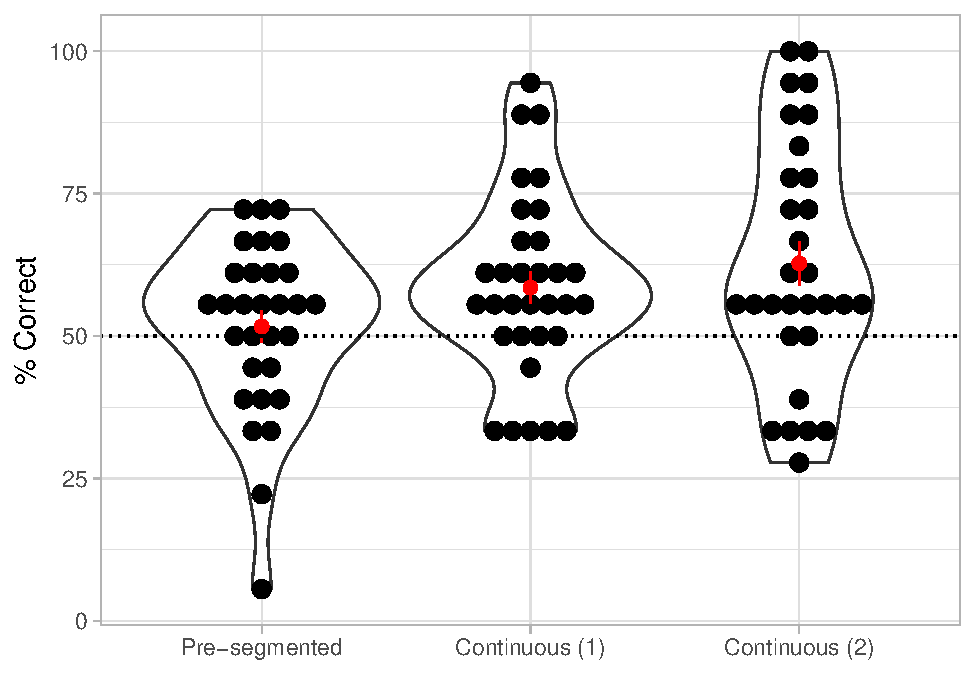
\includegraphics[width=0.8\linewidth]{segmentation_recall_combined_files/figure-latex/stats-london-stats.3x.us.segm.cont.plot-1} 

}

\caption{Results of Experiment 1. Each dot represents a participants. The central red dot is the sample mean; error bars represent standard errors from the mean. The results show the percentage of correct choices in the recognition test after familiarization with (left) a pre-segmented familiarization stream or (middle, right) a continuous familiarization stream. The two continuous conditions are replictions of one another.}\label{fig:stats-london-stats.3x.us.segm.cont.plot}
\end{figure}

\begin{table}

\caption{\label{tab:stats-london-stats.us.lang.glmm.print}Performance differences across familiarization conditions. The differences were assessed using a generalized linear model for the trial-by-trial data, using participants, correct items and foils as random factors. Random factors were removed from the model when they did not contribute to the model likelihood.}
\centering
\begin{tabular}[t]{lrrlrr}
\toprule
Effect & Estimate & Std. Error & CI & t & p\\
\midrule
\addlinespace[0.3em]
\multicolumn{6}{l}{\textbf{Pre-segmented familiarization}}\\
\hspace{1em}langL2 & 0.114 & 0.673 & -1.2, 1.43 & 0.170 & 0.865\\
\addlinespace[0.3em]
\multicolumn{6}{l}{\textbf{Continuous familiarization (1)}}\\
\hspace{1em}langL2 & -0.184 & 0.480 & -1.12, 0.757 & -0.383 & 0.702\\
\addlinespace[0.3em]
\multicolumn{6}{l}{\textbf{Continuous familiarization (2)}}\\
\hspace{1em}langL2 & 0.317 & 0.786 & -1.22, 1.86 & 0.403 & 0.687\\
\addlinespace[0.3em]
\multicolumn{6}{l}{\textbf{Pre-segmented vs. continuous familiarization (1)}}\\
\hspace{1em}langL2 & -0.019 & 0.557 & -1.11, 1.07 & -0.033 & 0.973\\
\hspace{1em}segmsegmented & -0.328 & 0.188 & -0.696, 0.0391 & -1.752 & 0.080\\
\addlinespace[0.3em]
\multicolumn{6}{l}{\textbf{Pre-segmented vs. continuous familiarization (2)}}\\
\hspace{1em}langL2 & 0.215 & 0.657 & -1.07, 1.5 & 0.327 & 0.743\\
\hspace{1em}segmsegmented & -0.608 & 0.244 & -1.09, -0.13 & -2.493 & 0.013\\
\bottomrule
\end{tabular}
\end{table}

\clearpage

\subsection{Recall experiment}\label{recall-experiment-2}

In the analyses below, we removed all items that contained syllables not
attested in the speech stream as it is unclear how these items should be
analyzed. As a result, we also removed participants who did not produce
any items that contained attested syllables only.

\begin{table}[!h]

\caption{\label{tab:recall-print-used-column-attributes}Analyses performed for the vocalizations}
\centering
\resizebox{\linewidth}{!}{
\begin{tabular}[t]{l>{\raggedright\arraybackslash}p{30em}}
\toprule
colName & meaning\\
\midrule
n.items & Number of recalled items\\
n.syll & Mean number of syllables of the recalled items\\
n.words & Number of recalled words\\
p.words & Proportion (among recalled items) of words\\
n.words.or.multiple & Number of recalled words or concatenation of words\\
\addlinespace
p.words.or.multiple & Proportion (among recalled items) of words or concatenation of words\\
n.part.words & Number of recalled part-words\\
p.part.words & Proportion (among recalled items) of part-words\\
n.part.words.or.multiple & Number of recalled part-words or concatenation of part-words\\
p.part.words.or.multiple & Proportion (among recalled items) of part-words or concatenation of part-words\\
\addlinespace
p.words.part.words & Proportion of words among (recalled) words and part-words. This is used for comparison to the recognition test.\\
p.words.part.words.or.multiple & Proportion of words among (recalled) words and part-words or concatenation thereof. This is used for comparison to the recognition test.\\
n.high.tp.chunk & Number of high TP chunks. High TP chunks are defined as two-syllabic chunk from a word\\
p.high.tp.chunk & Proprtion (among recalled items) of high TP chunks. High TP chunks are defined as two-syllabic chunk from a word\\
n.low.tp.chunk & Number of low TP chunks. Low TP chunks are defined as two-syllabic word transitions\\
\addlinespace
p.low.tp.chunk & Proportion (among recalled items) of low TP chunks. Low TP chunks are defined as two-syllabic word transitions\\
p.high.tp.chunk.low.tp.chunk & Proportion of high-TP chunks among high and low-TP chunks. High TP Chunks are defined as two-syllabic chunks from words; low TP chunks are two-syllabic word transitions\\
average\_fw\_tp & Average (across recalled items) of average forward TPs among transitions in a given item.\\
average\_fw\_tp\_d\_actual\_expected & Average (across recalled items) of the difference between the average ACTUAL forward TPs among transitions in a given item and the EXPECTED forward TP in that item, based on the items first element. See calculate.expected.tps.for.chunks for the calculations\\
average\_bw\_tp & Average (across recalled items) of average backward TPs among transitions in a given item.\\
\addlinespace
p.correct.initial.syll & Proportion (among recalled items) that have a correct initial syllable.\\
p.correct.final.syll & Proportion (among recalled items) that have a correct final syllable.\\
p.correct.initial.or.final.syll & Proportion (among recalled items) that have a correct initial or final syllable.\\
\bottomrule
\end{tabular}}
\end{table}

After computing these counts and averages, we asked which counts were
significantly different from zero in a one-tailed Wilcoxon test, either
for the continuous or the segmented condition. These counts were
n.items, n.syll, n.words, n.words.or.multiple, n.part.words,
n.part.words.or.multiple, n.high.tp.chunk, n.low.tp.chunk. (Note: These
counts are currently restricted to the testable data set.)

As shown in Table \ref{tab:recall-all-results-print}, participants
produced on average 1.338 words in the segmented condition, and 0.156 in
the continuous condition.

\subsubsection{General measures}\label{general-measures}

We first calculate the number of items produced as well their average,
and compare them against the zero as well as across segmentation
conditions. As shown in Table \ref{tab:recall-all-results-print} and
Figures \ref{fig:recall-general-measures-tp-plot}a and b, participants
produced positive number of items. Neither the number of items produced
nor their number of syllables differed across the segmentation
conditions.

\subsubsection{TP-based analyses}\label{tp-based-analyses}

We first computed the average forward TPs in the produced items, and
separately for each segmentation condition, compared it to both the
expected TPs for random strings and the expected TPs given the starting
syllable.

\begin{itemize}
\tightlist
\item
  The expected TPs for items of at least 2 syllables starting on an
  initial syllable are c(1, 1/3, 1, 1, 1/3, 1, 1, 1/3, \ldots{}). The
  difference between the actual and the expected TP needs to be compared
  to zero, as the expected TP differs across items.
\item
  The expected TPs for a random concatenation are the TPs in a random
  bigram. For an A or a B syllable, the random TP is 1 \(\times\) 1 /
  12, as there is only 1 (out of 12) non-zero TP continuations. For a C
  syllable, the random TP is 3 \(\times\) 1/3 / 12, as there are 3
  possible concatenations. On average, the random TP is thus
  \((1/12 + 1/12 + 1/12)/ 3 = 1/12 \approx .083\).
\end{itemize}

We compared these measures across segmentation conditions.

As shown in Table \ref{tab:recall-all-results-print} and Figures
\ref{fig:recall-general-measures-tp-plot}c and d, forward and backward
TPs were significantly greater than expected for a random string in both
the continuous and the segmented condition, with greater TPs in the
segmented conditions. However, they were significantly \emph{lower} than
the TPs expected if items recalled faithfully, given their starting
position.

As shown in Figure \ref{fig:recall-w-pw-chunks-positions-plot}b,
participants produced a positive number of high-TP chunks in both the
segmented and the continuous condition, with a significantly greater
number in the segmented condition. In contrast, they produced a positive
number of low-TP chunks only in the continuous condition. Accordingly,
the proportion of high-TP chunks among high- and low-TP chunks exceeded
50\% only in the segmented condition.

\subsubsection{Word vs.~part-word
analysis}\label{word-vs.part-word-analysis}

We next calculate the number and proportion of among (productions) of
words and part-words respectively; we also accept concatenations of
words and part-words. The proportions will be compared across stream
types as well as to zero.

Finally, we calculate the proportion of words among the word and
part-word productions. This proportion will be compared across
segmentation types, as well as to the chance level of 50\%.

As shown in Table \ref{tab:recall-all-results-print} and in Figure
\ref{fig:recall-w-pw-chunks-positions-plot}a, participants produced a
positive number of words only in the segmented condition, but not in the
continuous condition. In contrast, they produced a positive number of
part-words only in the continuous condition, but not in the segmented
condition. Accordingly, the proportion of words among words and
part-words was significantly greater than 50\% in the segmented
condition, but numerically (though not significantly) smaller than 50\%
in the continuous condition. The latter result is consistent with
participants randomly picking a syllable to start their vocalizations;
if so, part-words should be 2 times as likely as words.

\subsubsection{Positional analyses}\label{positional-analyses}

Finally, we analyze the productions in terms of correct initial final
positions. As there are four initial and final positions, respectively,
4/12 of the productions should have ``correct'' initial positions, 4/12
should have correct final positions, while
\(2 \times 4/12 - (4/12)^2 = 5/9\) should have either correct initial or
final positions.

As shown in Table \ref{tab:recall-all-results-print} and Figure
\ref{fig:recall-w-pw-chunks-positions-plot}c and d, participants
produced items with correct initial or final positions at great than
chance level only in the segmented condition, but not the continuous
condition.

\textbackslash{}begin\{table\}

\textbackslash{}caption\{\label{tab:recall-all-results-print}Various
analyses pertaining to the productions as well as test against their
chances levels. Number of items produced, their numbers of syllables,
number of words, number of part-words (chance level: 0), proportion of
words among productions, proportion of part-words among productions,
proportion of words among words and part-words (chance level 50\%),
average forward TPs (chance level: 1/12), difference between
positionally expected and actual TPs, average backward TPS. CHUNKS \}
\centering
\resizebox{\linewidth}{!}{
\begin{tabular}[t]{l>{\raggedright\arraybackslash}p{30em}>{\raggedright\arraybackslash}p{30em}>{\raggedleft\arraybackslash}p{10em}}
\toprule
 & Continuous & Segmented & *p* (Continuous vs. Segmented)\\
\midrule
\addlinespace[0.3em]
\multicolumn{4}{l}{\textbf{Recognition accuracy}}\\
\hspace{1em}lab-based & \M = 0.607, \SE = 0.0448, \p = 0.0477 & \M = 0.911, \SE = 0.0439, \p = 0.000898 & 0.008\\
\hspace{1em}online & \M = 0.595, \SE = 0.0335, \p = 0.00411 & \M = 0.887, \SE = 0.0268, \p = 5.38e-10 & 0.000\\
\addlinespace[0.3em]
\multicolumn{4}{l}{\textbf{Number of items}}\\
\hspace{1em}lab-based & \M = 4.21, \SE = 0.723, \p = 0.00106 & \M = 4.21, \SE = 0.763, \p = 0.00103 & 0.843\\
\hspace{1em}online & \M = 4.73, \SE = 0.315, \p = 4.75e-12 & \M = 3.69, \SE = 0.326, \p = 4.13e-10 & 0.013\\
\addlinespace[0.3em]
\multicolumn{4}{l}{\textbf{Number of syllables/item}}\\
\hspace{1em}lab-based & \M = 3.53, \SE = 0.453, \p = 0.00107 & \M = 2.8, \SE = 0.151, \p = 0.000546 & 0.053\\
\hspace{1em}online & \M = 2.27, \SE = 0.114, \p = 4.55e-12 & \M = 2.82, \SE = 0.0798, \p = 7.06e-11 & 0.000\\
\addlinespace[0.3em]
\multicolumn{4}{l}{\textbf{Proportion of words among words and part-words (or concatenations thereof)}}\\
\hspace{1em}lab-based & \M = 0.321, \SE = 0.153, \p = 0.322 (vs. 0.5); 0.798 (vs. 0.333333333333333) & \M = 1, \SE = 0, \p = 0.000627 (vs. 0.5); 0.000627 (vs. 0.333333333333333) & 0.034\\
\hspace{1em}online & \M = 0.357, \SE = 0.138, \p = 0.301 (vs. 0.5); 0.649 (vs. 0.333333333333333) & \M = 1, \SE = 0, \p = 9.79e-09 (vs. 0.5); 9.79e-09 (vs. 0.333333333333333) & 0.000\\
\addlinespace[0.3em]
\multicolumn{4}{l}{\textbf{Forward TPs}}\\
\hspace{1em}lab-based & \M = 0.301, \SE = 0.0702, \p = 0.0107 & \M = 0.634, \SE = 0.092, \p = 0.00159 & \vphantom{1} 0.006\\
\hspace{1em}online & \M = 0.372, \SE = 0.0361, \p = 4.4e-09 & \M = 0.555, \SE = 0.049, \p = 8.76e-09 & \vphantom{1} 0.004\\
\addlinespace[0.3em]
\multicolumn{4}{l}{\textbf{Backward TPs}}\\
\hspace{1em}lab-based & \M = 0.301, \SE = 0.0702, \p = 0.0107 & \M = 0.634, \SE = 0.092, \p = 0.00159 & 0.006\\
\hspace{1em}online & \M = 0.372, \SE = 0.0361, \p = 4.4e-09 & \M = 0.555, \SE = 0.049, \p = 8.76e-09 & 0.004\\
\addlinespace[0.3em]
\multicolumn{4}{l}{\textbf{Proportion of High-TP chunks among High- and Low-TP chunks}}\\
\hspace{1em}lab-based & \M = 0.75, \SE = 0.289, \p = 0.424 (vs. 0.5); 0.85 (vs. 0.666666666666667) & \M = 1, \SE = 0, \p = 0.000627 (vs. 0.5); 0.000627 (vs. 0.666666666666667) & 1.000\\
\hspace{1em}online & \M = 0.721, \SE = 0.0574, \p = 0.000702 (vs. 0.5); 0.0556 (vs. 0.666666666666667) & \M = 0.95, \SE = 0.0353, \p = 1.31e-08 (vs. 0.5); 6.14e-07 (vs. 0.666666666666667) & 0.000\\
\addlinespace[0.3em]
\multicolumn{4}{l}{\textbf{Proportion of items with correct initial syllables}}\\
\hspace{1em}lab-based & \M = 0.318, \SE = 0.0984, \p = 0.691 & \M = 0.789, \SE = 0.0666, \p = 0.00123 & 0.012\\
\hspace{1em}online & \M = 0.425, \SE = 0.0385, \p = 0.0357 & \M = 0.72, \SE = 0.045, \p = 3.7e-08 & 0.000\\
\addlinespace[0.3em]
\multicolumn{4}{l}{\textbf{Proportion of items with correct final syllables}}\\
\hspace{1em}lab-based & \M = 0.46, \SE = 0.116, \p = 0.48 & \M = 0.76, \SE = 0.0976, \p = 0.00275 & 0.045\\
\hspace{1em}online & \M = 0.369, \SE = 0.0438, \p = 0.781 & \M = 0.694, \SE = 0.0524, \p = 3.56e-07 & 0.000\\
\bottomrule
\end{tabular}} \textbackslash{}end\{table\}

\begin{figure}

{\centering 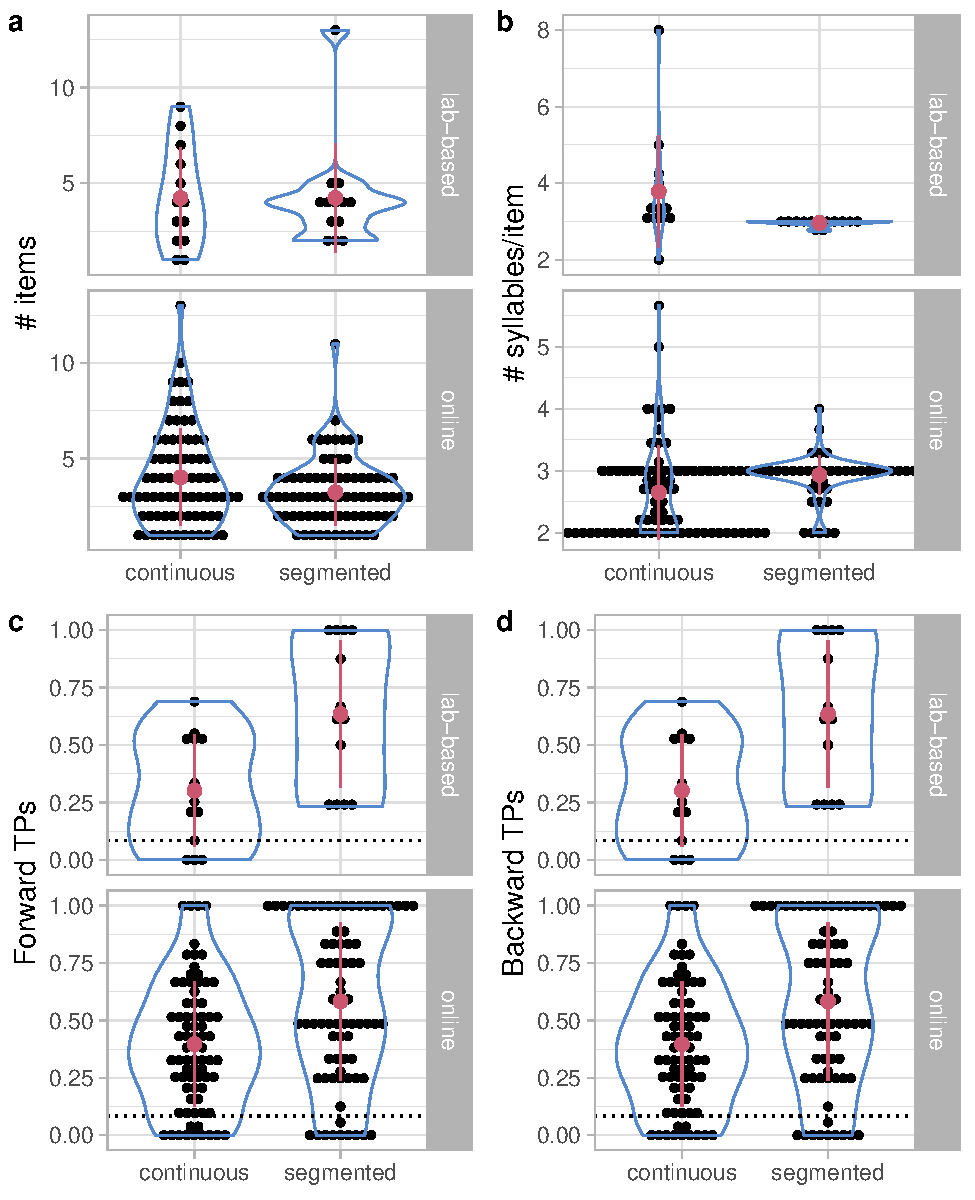
\includegraphics[width=0.8\linewidth]{segmentation_recall_combined_files/figure-latex/recall-general-measures-tp-plot-1} 

}

\caption{Number of items produced, number of syllables per item and forward and backward TPs. The dotted line represents the chance level for a randomly ordered syllable sequence.}\label{fig:recall-general-measures-tp-plot}
\end{figure}

\textbackslash{}begin\{figure\}

\{\centering 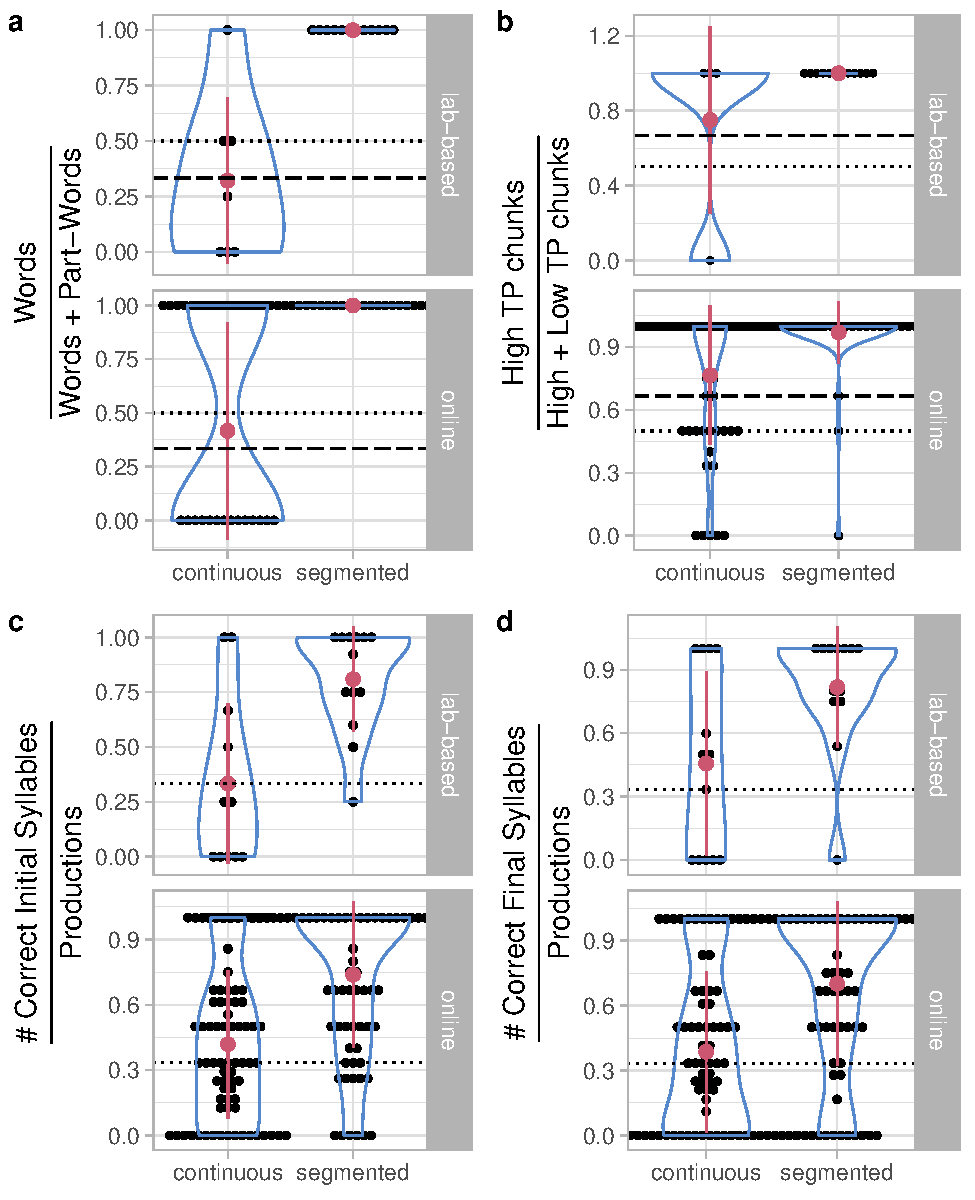
\includegraphics[width=0.8\linewidth]{segmentation_recall_combined_files/figure-latex/recall-w-pw-chunks-positions-plot-1}

\}

\textbackslash{}caption\{Analyses of the participants' productions. (a)
Proportion of words among words and part-words. The dotted line
represents the chance level of 50\% in a two-alternative forced-choice
task, while the dashed line represents the chance level of 33\% that an
attested 3 syllable-chunk is a word rather than a part-word. (b)
Proportion of high-TP chunks among high- and low-TP chunks. The dashed
line represents the chance level of 66\% that an attested 2
syllable-chunk is a high-TP rather than a low-TP chunk. (c) proportion
of productions with correct initial syllables and (d) with correct final
syllables. The dotted line represents the chance level of
33\%.\}\label{fig:recall-w-pw-chunks-positions-plot}
\textbackslash{}end\{figure\}

\clearpage

\section{Appendix}\label{appendix}

\subsection{Additional results for the recall
experiments}\label{additional-results-for-the-recall-experiments}

\textbackslash{}begin\{table\}

\textbackslash{}caption\{\label{tab:recall-extra-results-print}Various
supplementary analyses pertaining to the productions as well as test
against their chances levels. Number of items produced, their numbers of
syllables, number of words, number of part-words (chance level: 0),
proportion of words among productions, proportion of part-words among
productions, proportion of words among words and part-words (chance
level 50\%), average forward TPs (chance level: 1/12), difference
between positionally expected and actual TPs, average backward TPS.
CHUNKS \} \centering
\resizebox{\linewidth}{!}{
\begin{tabular}[t]{l>{\raggedright\arraybackslash}p{30em}>{\raggedright\arraybackslash}p{30em}>{\raggedleft\arraybackslash}p{10em}}
\toprule
 & Continuous & Segmented & *p* (Continuous vs. Segmented)\\
\midrule
\addlinespace[0.3em]
\multicolumn{4}{l}{\textbf{Number of words}}\\
\hspace{1em}lab-based & \M = 0.286, \SE = 0.13, \p = 0.0719 & \M = 1.71, \SE = 0.316, \p = 0.00224 & \vphantom{1} 0.005\\
\hspace{1em}online & \M = 0.143, \SE = 0.0752, \p = 0.0545 & \M = 1.24, \SE = 0.18, \p = 3.63e-07 & \vphantom{1} 0.000\\
\addlinespace[0.3em]
\multicolumn{4}{l}{\textbf{Proportion of words among productions}}\\
\hspace{1em}lab-based & \M = 0.286, \SE = 0.13, \p = 0.0719 & \M = 1.71, \SE = 0.316, \p = 0.00224 & 0.005\\
\hspace{1em}online & \M = 0.143, \SE = 0.0752, \p = 0.0545 & \M = 1.24, \SE = 0.18, \p = 3.63e-07 & 0.000\\
\addlinespace[0.3em]
\multicolumn{4}{l}{\textbf{Number of part-words}}\\
\hspace{1em}lab-based & \M = 0.643, \SE = 0.258, \p = 0.031 & \M = 0, \SE = 0, \p = NaN & \vphantom{1} 0.031\\
\hspace{1em}online & \M = 0.19, \SE = 0.0639, \p = 0.00693 & \M = 0, \SE = 0, \p = NaN & \vphantom{1} 0.005\\
\addlinespace[0.3em]
\multicolumn{4}{l}{\textbf{Proportion of part-words among productions}}\\
\hspace{1em}lab-based & \M = 0.643, \SE = 0.258, \p = 0.031 & \M = 0, \SE = 0, \p = NaN & 0.031\\
\hspace{1em}online & \M = 0.19, \SE = 0.0639, \p = 0.00693 & \M = 0, \SE = 0, \p = NaN & 0.005\\
\addlinespace[0.3em]
\multicolumn{4}{l}{\textbf{Actual vs. expected forward TPs}}\\
\hspace{1em}lab-based & \M = -0.513, \SE = 0.0814, \p = 0.000244 & \M = -0.328, \SE = 0.0823, \p = 0.00909 & 0.126\\
\hspace{1em}online & \M = -0.462, \SE = 0.0385, \p = 2.57e-10 & \M = -0.38, \SE = 0.043, \p = 3.66e-08 & 0.156\\
\addlinespace[0.3em]
\multicolumn{4}{l}{\textbf{Number of High-TP chunks}}\\
\hspace{1em}lab-based & \M = 0.714, \SE = 0.427, \p = 0.181 & \M = 2.14, \SE = 0.375, \p = 0.00224 & 0.022\\
\hspace{1em}online & \M = 1.02, \SE = 0.14, \p = 6.57e-08 & \M = 1.53, \SE = 0.193, \p = 5.53e-08 & 0.039\\
\addlinespace[0.3em]
\multicolumn{4}{l}{\textbf{Proportion of High-TP chunks among productions}}\\
\hspace{1em}lab-based & \M = 0.097, \SE = 0.056, \p = 0.181 & \M = 0.561, \SE = 0.102, \p = 0.00241 & 0.003\\
\hspace{1em}online & \M = 0.208, \SE = 0.0311, \p = 1.12e-07 & \M = 0.432, \SE = 0.0485, \p = 7.19e-08 & 0.000\\
\addlinespace[0.3em]
\multicolumn{4}{l}{\textbf{Number of Low-TP chunks}}\\
\hspace{1em}lab-based & \M = 0.0714, \SE = 0.0741, \p = 1 & \M = 0, \SE = 0, \p = NaN & 1.000\\
\hspace{1em}online & \M = 0.365, \SE = 0.0832, \p = 8.81e-05 & \M = 0.0588, \SE = 0.0439, \p = 0.371 & 0.001\\
\addlinespace[0.3em]
\multicolumn{4}{l}{\textbf{Number of Low-TP chunks among productions}}\\
\hspace{1em}lab-based & \M = 0.00893, \SE = 0.00927, \p = 1 & \M = 0, \SE = 0, \p = NaN & 1.000\\
\hspace{1em}online & \M = 0.0692, \SE = 0.0165, \p = 0.000206 & \M = 0.00915, \SE = 0.00706, \p = 0.371 & 0.001\\
\bottomrule
\end{tabular}} \textbackslash{}end\{table\}

\begin{figure}

{\centering 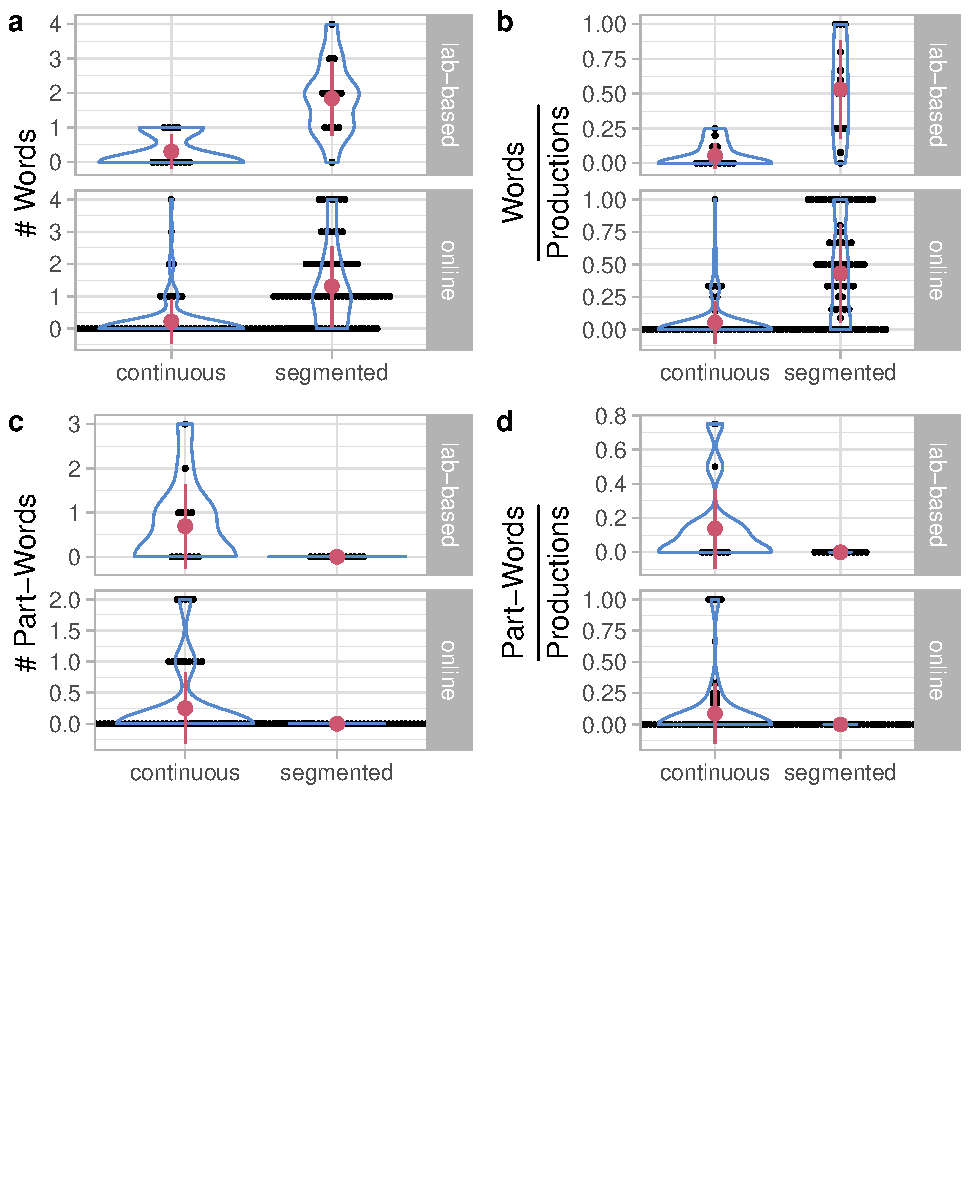
\includegraphics[width=0.8\linewidth]{segmentation_recall_combined_files/figure-latex/recall-words-part-words-raw-plot-1} 

}

\caption{Number and proportion (among vocalizations) of words and part-words.}\label{fig:recall-words-part-words-raw-plot}
\end{figure}

\begin{figure}

{\centering 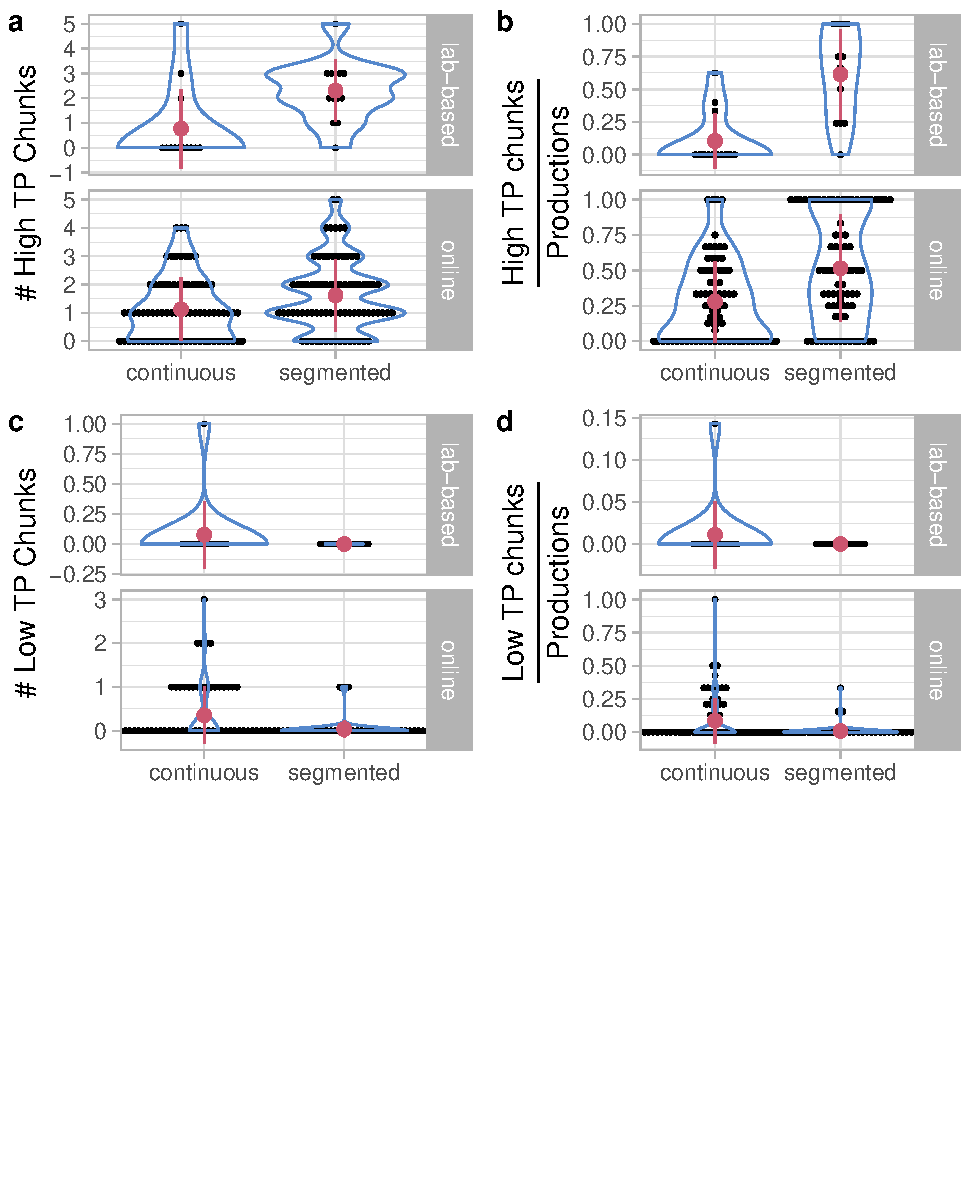
\includegraphics[width=0.8\linewidth]{segmentation_recall_combined_files/figure-latex/recall-tp-chunks-raw-plot-1} 

}

\caption{Plot of High and Low TP chunks.}\label{fig:recall-tp-chunks-raw-plot}
\end{figure}

\clearpage

\subsection{\texorpdfstring{Experiments with the \emph{en1} diphone
base}{Experiments with the en1 diphone base}}\label{experiments-with-the-en1-diphone-base}

\subsubsection{Segmented stream, 3 repetitions of the stream, en1
diphone
based}\label{segmented-stream-3-repetitions-of-the-stream-en1-diphone-based}

\begin{figure}

{\centering 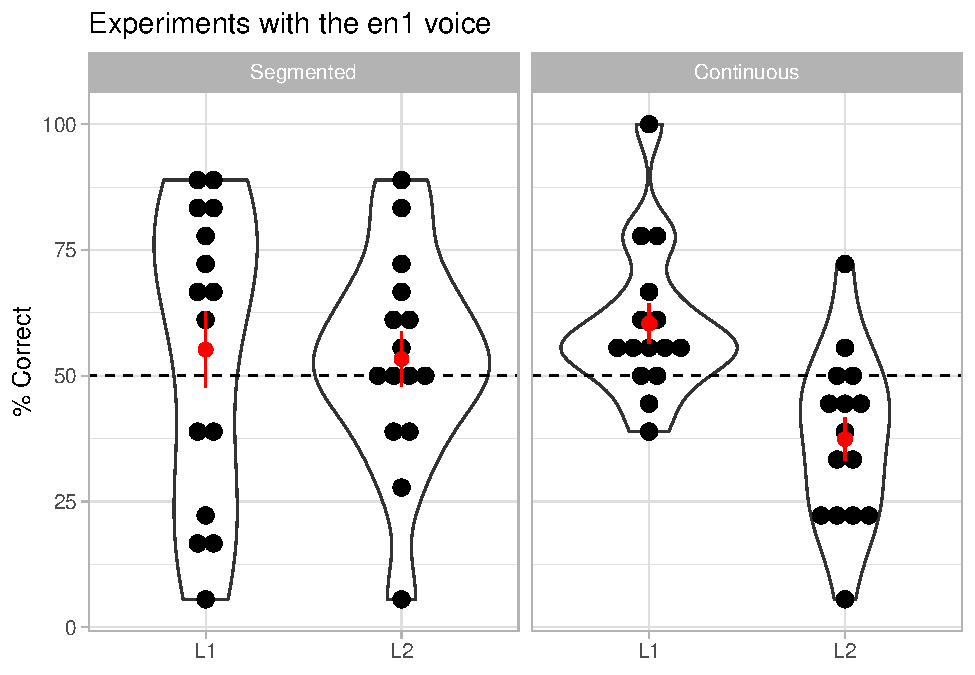
\includegraphics[width=0.8\linewidth]{segmentation_recall_combined_files/figure-latex/stats-london-stats.3x.en.segm-cont.plot-1} 

}

\caption{Results for a pre-segmented presentation of the stream (540 ms silences, left) and continuous presentation of the stream (right). Each word was repeated 45 times. The diphone based was *en1*.}\label{fig:stats-london-stats.3x.en.segm-cont.plot}
\end{figure}

As shown in Figure \ref{fig:stats-london-stats.3x.en.segm-cont.plot},
the average performance did not differ significantly from the chance
level of 50\%, (\M\textasciitilde{}= 54.26, \SD\textasciitilde{}=
25.09), \T(29) = 0.93, \p\textasciitilde{}= 0.36, \D\textasciitilde{}=
0.17, \CI\textasciitilde{}= 44.89, 63.63, ns, . Likelihood ratio
analysis favored the null hypothesis by a factor of 3.555 after
correction with the Bayesian Information Criterion. Further, as shown in
Table \ref{tab:stats.en.lang.glmm}, performance did not depend on the
language condition.

\subsubsection{Continuous stream, 3 repetitions of the stream, en1
diphone
based}\label{continuous-stream-3-repetitions-of-the-stream-en1-diphone-based}

As shown in Figure \ref{fig:stats-london-stats.3x.en.segm-cont.plot},
the average performance did not differ significantly from the chance
level of 50\%, (\M\textasciitilde{}= 48.89, \SD\textasciitilde{}=
19.65), \T(29) = -0.31, \p\textasciitilde{}= 0.759, \D\textasciitilde{}=
0.057, \CI\textasciitilde{}= 41.55, 56.23, ns, \(V\) = 166, \(p\) =
0.818. Likelihood analyses revealed that the null hypothesis was 5.221
than the alternative hypothesis after a correction with the Bayesian
Information Criterion. However, as shown in Table
\ref{tab:stats.en.lang.glmm}, performance was much better for Language 1
than for Language 2, presumably due to some click-like sounds the
synthesizer produced for some stops and fricatives (notably /f/ and
/g/). These sound might have prevent participants from using statistical
learning.

\begin{table}

\caption{\label{tab:stats-london-stats.en.lang.glmm.print}\label{tab:stats.en.lang.glmm}Performance differences across language conditions. The differences were assessed using a generalized linear model for the trial-by-trial data, using participants, correct items and foils as random factors. Random factors were removed from the model when they did not contribute to the model likelihood}
\centering
\begin{tabular}[t]{lrrlrr}
\toprule
Effect & Estimate & Std. Error & CI & t & p\\
\midrule
\addlinespace[0.3em]
\multicolumn{6}{l}{\textbf{stats.3x.en.segm}}\\
\hspace{1em}langL2 & -0.097 & 0.441 & -0.96, 0.767 & -0.22 & 0.826\\
\addlinespace[0.3em]
\multicolumn{6}{l}{\textbf{stats.3x.en.cont}}\\
\hspace{1em}langL2 & -1.024 & 0.410 & -1.83, -0.22 & -2.50 & 0.013\\
\bottomrule
\end{tabular}
\end{table}

\subsection{Pilot recognition experiment testing the use of chunk
frequency}\label{pilot-recognition-experiment-testing-the-use-of-chunk-frequency}

In Pilot Experiment 1, we asked if participants could break up
tri-syllabic items by using the chunk frequency of sub-chunks. The
artificial languages were designed such that, in a trisyllabic item such
as \emph{ABC}, chunk frequency (and backwards TPs) favor in the initial
\emph{AB} chunk for half of the participants, and the final \emph{BC}
chunk for the other participants.

Across participants, we also varied the exposure to the languages, with
3, 15 or 30 repetitions per word, respectively.

\subsubsection{Methods}\label{methods-1}

\paragraph{Participants}\label{participants-1}

\begin{table}

\caption{\label{tab:bcn-demographics}Demographics of Pilot Experiment 1.}
\centering
\begin{tabular}[t]{rrrl}
\toprule
\# Repetitions/word & *N* & Age (*M*) & Age (Range)\\
\midrule
3 & 37 & 21.1 & 18-35\\
15 & 41 & 21.0 & 18-27\\
30 & 40 & 20.8 & 18-26\\
\bottomrule
\end{tabular}
\end{table}

Demographic information of Pilot Experiment 1 is given in Table
\ref{tab:bcn-demographics}. Participants were native speakers of Spanish
and Catalan and were recruited from the Universitat Pompeu Fabra
community.

\subsubsection{Stimuli}\label{stimuli-1}

Stimuli transcriptions are given in Table
\ref{tab:bcn-print-language-structure}. They were synthesized using the
\emph{es2} (Spanish male) diphone base of the mbrola \citep{mbrola}
speech synthesized, using a segment duration of 225 ms and an
fundamental frequency of 120 Hz.

\paragraph{Apparatus}\label{apparatus-1}

Participants were test individually in a quiet room. Stimuli were
presented over headphones. Responses were collected from pre-marked keys
on the keyboard. The experiment with 3 repetitions per word (see below)
were run using PsyScope X; the other experiments were run using
Experyment (\url{https://www.expyriment.org/}).

\paragraph{Familiarization}\label{familiarization-1}

The design of Pilot Experiment 1 is shown in Table
\ref{tab:bcn-print-language-structure}. The languages comprise
trisyllabic items. All foward TPs were 0.5. However, in Language 1 the
chunk composed of the first two syllables (e.g., \emph{AB} in
\emph{ABC}) were twice as frequent as the chunk composed of the last two
syllables (e.g., \emph{BC} in \emph{ABC}); the backward TPs were twice
as high as well. Language 2 favored the word-final chunk. Participants
were informed that they would listen to a sequency of Martian words, and
then listened to a sequence of the eight words in
\ref{tab:stats-london-print-language-structure} with an ISI of 1000 ms
and 3, 15 or 30 repetitions per word. Due to programming error, the
familiarization items for 15 and 30 repetitions per word were sampled
with replacement.

\begin{table}

\caption{\label{tab:bcn-print-language-structure}Design of the Pilot Experiment 1. (Left) Language structure. (Middle) Structure of test items. Correct items for Language 1 are foils for Language 2 and vice versa. (Right) Actual items in SAMPA format; dashes indicate syllable boundaries}
\centering
\begin{tabular}[t]{llllll}
\toprule
\multicolumn{2}{c}{Word structure for} & \multicolumn{2}{c}{Test item structure for} & \multicolumn{2}{c}{Actual words for} \\
Language 1 & Language 2 & Language 1 & Language 2 & Language 1 & Language 2\\
\midrule
ABC & ABC & AB & BC & ka-lu-mo & ka-lu-mo\\
DEF & DEF & DE & EF & ne-fi-To & ne-fi-To\\
ABF & DBC &  &  & ka-lu-To & ne-lu-mo\\
DEC & AEF &  &  & ne-fi-mo & ka-fi-To\\
AGJ & JBG &  &  & ka-do-ri & ri-lu-do\\
\addlinespace
AGK & KBG &  &  & ka-do-tSo & tSo-lu-do\\
DHJ & JEH &  &  & ne-pu-ri & ri-fi-pu\\
DHK & KEH &  &  & ne-pu-tSo & tSo-fi-pu\\
\bottomrule
\end{tabular}
\end{table}

\paragraph{Test}\label{test}

Following this familiarization, participants were informed that they
would hear new items, and had to decide which of them was in Martian.
Following this, they heard pairs of two syllabic items with an ISI of
1000 ms. One was a word-initial chunk and one a word-final chunk.

The test items shown in Table
\ref{tab:stats-london-print-language-structure} were combined into four
test pairs, which were presented twice with different item orders. A new
trial started 100 ms after a participant response.

\subsubsection{Results}\label{results-1}

\begin{figure}

{\centering 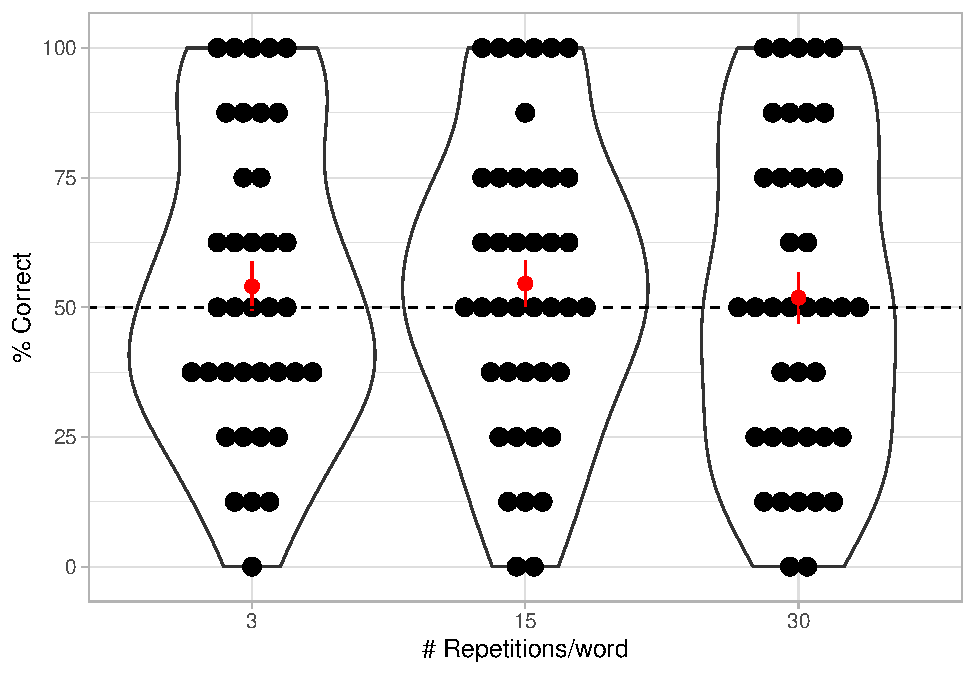
\includegraphics[width=0.8\linewidth]{segmentation_recall_combined_files/figure-latex/bcn-plot-stats-1} 

}

\caption{Results of Pilot Experiment 1. Each dot represents a participants. The central red dot is the sample mean; error bars represent standard errors from the mean. The results show the percentage of correct choices in the recognition test after familiarization with (left) 3, (middle) 15  or (right) 30 repetitions per word.}\label{fig:bcn-plot-stats}
\end{figure}

\begin{table}

\caption{\label{tab:bcn-glmm-print}Performance in Pilot Experiment 1 for different amounts of exposure. The differences were assessed using a generalized linear model for the trial-by-trial data, using participants as a random factor.}
\centering
\begin{tabular}[t]{lrrlrr}
\toprule
Effect & Estimate & Std. Error & CI & t & p\\
\midrule
langL2 & 0.337 & 0.493 & -0.629, 1.3 & 0.684 & 0.494\\
n.rep.word & 0.017 & 0.018 & -0.018, 0.0513 & 0.942 & 0.346\\
langL2:n.rep.word & -0.042 & 0.025 & -0.0916, 0.00698 & -1.682 & 0.093\\
\bottomrule
\end{tabular}
\end{table}

As shown Table \ref{tab:bcn-glmm-print}, a generalized linear model
revealed that performance depended neither on the amount of
familiarization nor on the familiarization language. As shown in Figure
\ref{fig:bcn-plot-stats}, a Wilcoxon test did not detect any deviation
from the chance level of 50\%, neither for all amounts of
familiarization combined, \M = 53.5, \SE = 2.71, \p = 0.182, nor for the
individual familiarization conditions (3 repetitions per word: \M =
54.1, \SE = 4.81, \p = 0.416; 15 repetitions per word: \M = 54.6, \SE =
4.52, \p = 0.325; 30 repetitions per word: \M = 51.9, \SE = 4.98, \p =
0.63). Following \citet{Glover2004}, the null hypothesis was 4.696 times
more likely than the alternative hypothesis after corrections with the
Bayesian Information Criterion, and 1.217 more likely after correction
with the Akaike Information Criterion.

\clearpage

\bibliography{/Users/endress/ansgar.bib,/Users/endress/ansgar.own.bib}

\end{document}
